\documentclass{article}

\usepackage{graphicx}
\usepackage{rotating}
\usepackage{amsmath}
\usepackage{amssymb}
\usepackage{fancyhdr}
\usepackage{listings}
%\usepackage{xcolor}
\usepackage{color}
\usepackage{amsfonts}
\usepackage{textcomp}
\usepackage{float}
\usepackage[sorting=none]{biblatex}
\usepackage[margin=1in]{geometry}
\usepackage[font={small,it}]{caption}
\usepackage[table,xcdraw]{xcolor}
\usepackage{placeins}
\usepackage{xepersian}





%\DeclareMathOperator*{\btie}{\bowtie}
\addbibresource{bibliography.bib}
\settextfont[Scale=1.2]{B-NAZANIN.TTF}
\setlatintextfont[Scale=1]{Times New Roman}
\renewcommand{\baselinestretch}{1.5}
\pagestyle{fancy}
\fancyhf{}
\rhead{تکلیف دوم درس مبانی رمزنگاری}
\lhead{\thepage}
\rfoot{علیرضا ابره فروش}
\lfoot{9816603}
\renewcommand{\headrulewidth}{1pt}
\renewcommand{\footrulewidth}{1pt}
%%%%%%%%%%
\lstset
{
    language=[latex]tex,
    basicstyle=\ttfamily,
    commentstyle=\color{black},
    columns=fullflexible,
    keepspaces=true,
    upquote=true,
    showstringspaces=false,
    morestring=[s]\\\%,
    stringstyle=\color{black},
}
%%%%%%%%%%
%beginMatlab
\definecolor{mygreen}{RGB}{28,172,0} % color values Red, Green, Blue
\definecolor{mylilas}{RGB}{170,55,241}
%endMatlab
\begin{document}
%beginMatlab
\lstset{language=Matlab,%
    %basicstyle=\color{red},
    breaklines=true,%
    morekeywords={matlab2tikz},
    keywordstyle=\color{blue},%
    morekeywords=[2]{1}, keywordstyle=[2]{\color{black}},
    identifierstyle=\color{black},%
    stringstyle=\color{mylilas},
    commentstyle=\color{mygreen},%
    showstringspaces=false,%without this there will be a symbol in the places where there is a space
    numbers=left,%
    numberstyle={\tiny \color{black}},% size of the numbers
    numbersep=9pt, % this defines how far the numbers are from the text
    emph=[1]{for,end,break},emphstyle=[1]\color{red}, %some words to emphasise
    %emph=[2]{word1,word2}, emphstyle=[2]{style},    
}
%endMatlab
\begin{titlepage}
\begin{center}

\includegraphics[width=0.4\textwidth]{figures/IUT Logo.png}\\
        
\LARGE
\textbf{دانشگاه صنعتی اصفهان}\\
\textbf{دانشکده مهندسی برق و کامپیوتر}\\
        
\vfill
        
\huge
\textbf{عنوان: تکلیف چهارم درس ریزپردازنده}\\
        
\vfill
        
\LARGE
\textbf{نام و نام خانوادگی: علیرضا ابره فروش}\\
\textbf{شماره دانشجویی: 9816603}\\
\textbf{نیم\,سال تحصیلی: پاییز 1400}\\
\textbf{مدرّس: دکتر عارف کریمی افشار}\\
\end{center}
\end{titlepage}


%\tableofcontents
\newpage


\section{}%1
\begin{latin}
"One-time pad is a cryptographic encryption technique that uses a random key that is as long as the message itself. The key is used only once, and both the sender and receiver must have a copy of the same key to encrypt and decrypt messages. Here are some pros and cons of one-time pad:\\
Pros:
\begin{enumerate}

    \item Security: One-time pad encryption is considered to be unbreakable if used correctly, as it provides perfect secrecy. The encryption key used is completely random and cannot be guessed or predicted, making it virtually impossible for an attacker to break.

    \item Simplicity: One-time pad encryption is simple to understand and implement, as it involves only the use of a random key and the XOR operation. It does not require complex algorithms or mathematical computations, making it a preferred choice for encrypting short messages.

    \item Privacy: One-time pad encryption ensures complete privacy, as it does not reveal any information about the original message, even if an attacker intercepts the ciphertext.
\end{enumerate}
Cons:
\begin{enumerate}
    \item Key distribution: One-time pad encryption requires both the sender and the receiver to have a copy of the same key. This can be challenging in practice, especially if the keys need to be distributed securely over long distances.

    \item Key management: The one-time pad key can be used only once and must be discarded after use, making key management a challenge. Generating a truly random key that is as long as the message itself can also be difficult.

    \item Size limitations: One-time pad encryption requires a key that is as long as the message, which can make it impractical for encrypting large amounts of data.

    \item Vulnerable to certain attacks: One-time pad encryption is vulnerable to certain attacks, such as key reuse or guessing attacks, which can compromise the security of the encryption."
\end{enumerate}
\end{latin}

\section{}%2
\subsection{}
\begin{latin}
\begin{enumerate}
\item LFSRs which generate a maximum-length sequence. These LFSRs are based on
primitive polynomials.
\item LFSRs which do not generate a maximum-length sequence but whose sequence
length is independent of the initial value of the register. These LFSRs are based
on irreducible polynomials that are not primitive. Note that all primitive polynomials are also irreducible.
\item LFSRs which do not generate a maximum-length sequence and whose sequence
length depends on the initial values of the register. These LFSRs are based on
reducible polynomials.
\end{enumerate}
\end{latin}

\subsection{}
\subsubsection{}
\begin{latin}
$
P\left( x \right) = x ^ 4 + x ^ 3 + x ^ 2 + x + 1\\
m = 4\\
p_3 = p_2 = p_1 = p_0 = 1
$
\end{latin}
\begin{figure}[H]
    \centering
    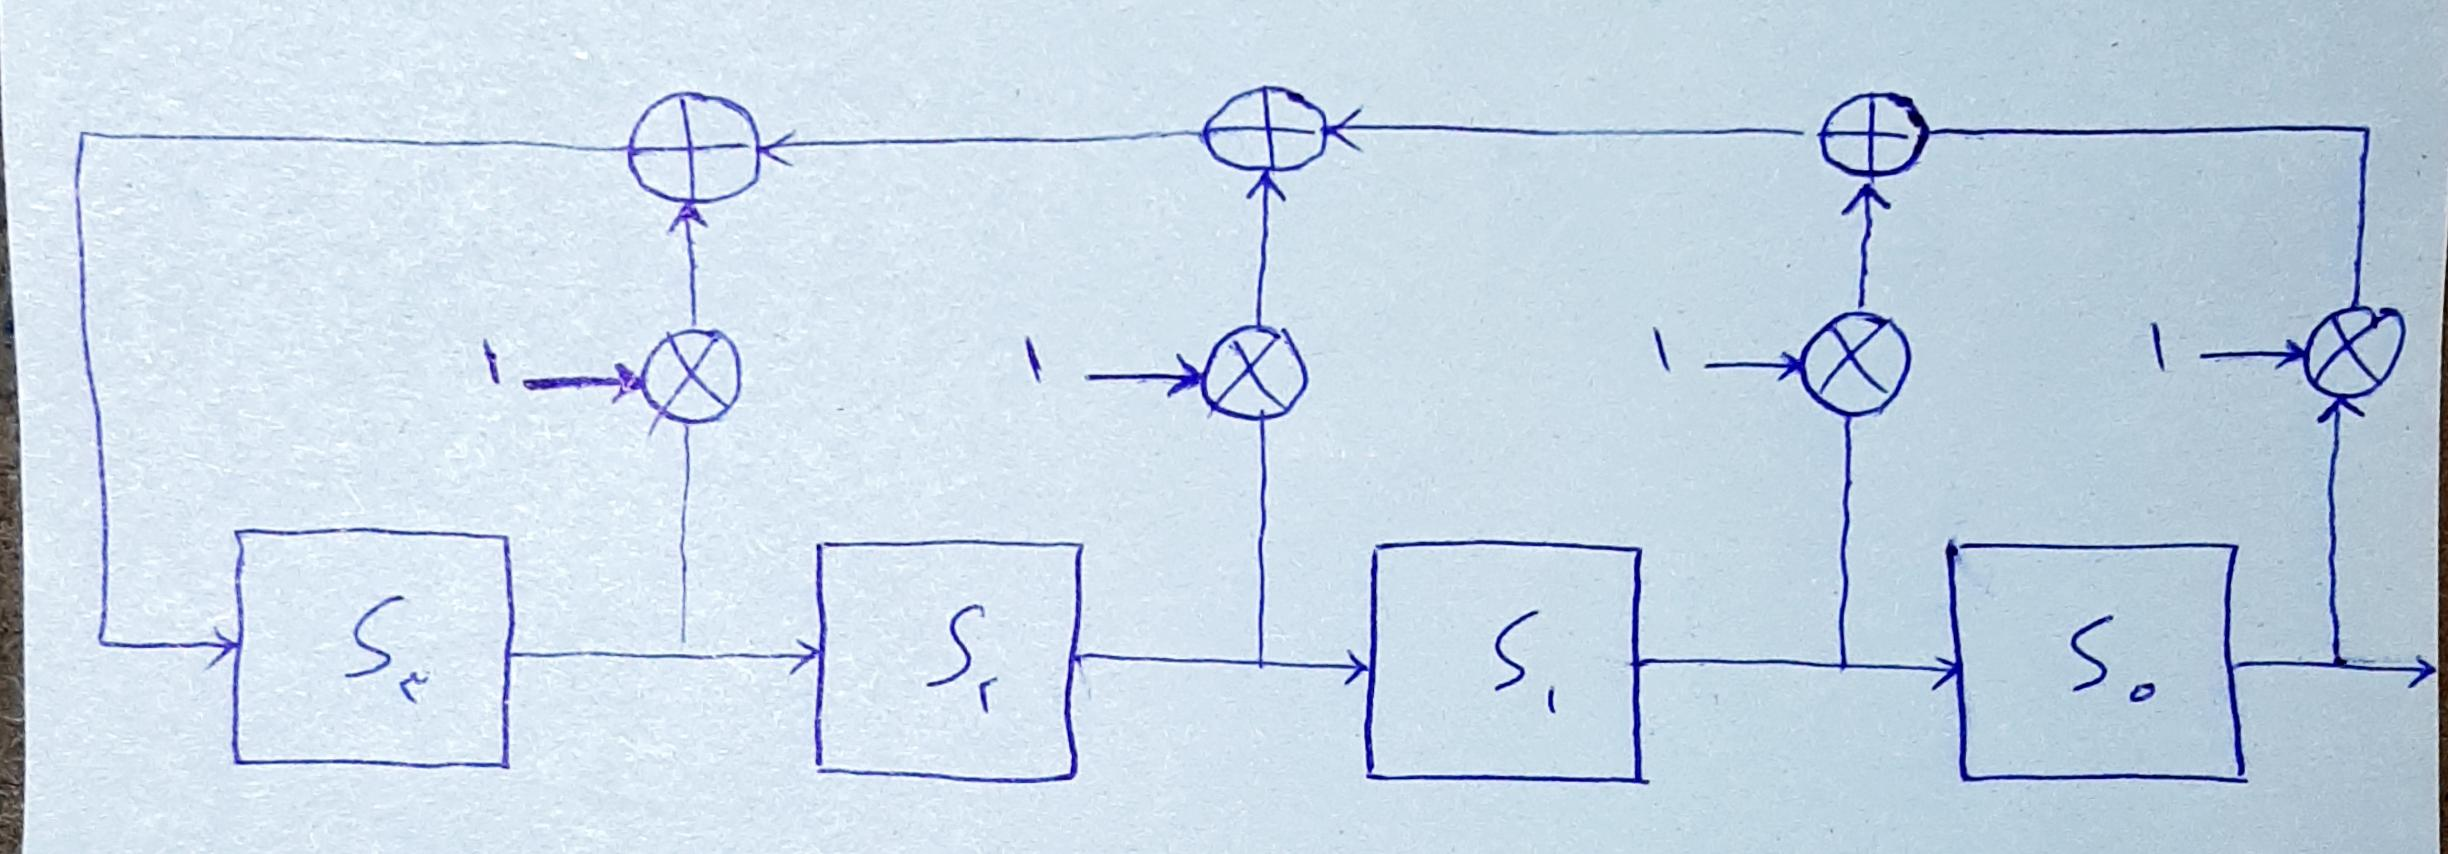
\includegraphics[width=0.75\textwidth]{figures/1.jpg}
    \caption
	{}
    \label{fig:fig1}
\end{figure}

\subsubsection{}
\begin{latin}
$
P\left( x \right) = x ^ 3 + x + 1\\
m = 3\\
p_2 = 0,  p_1 = p_0 = 1
$
\end{latin}
\begin{figure}[H]
    \centering
    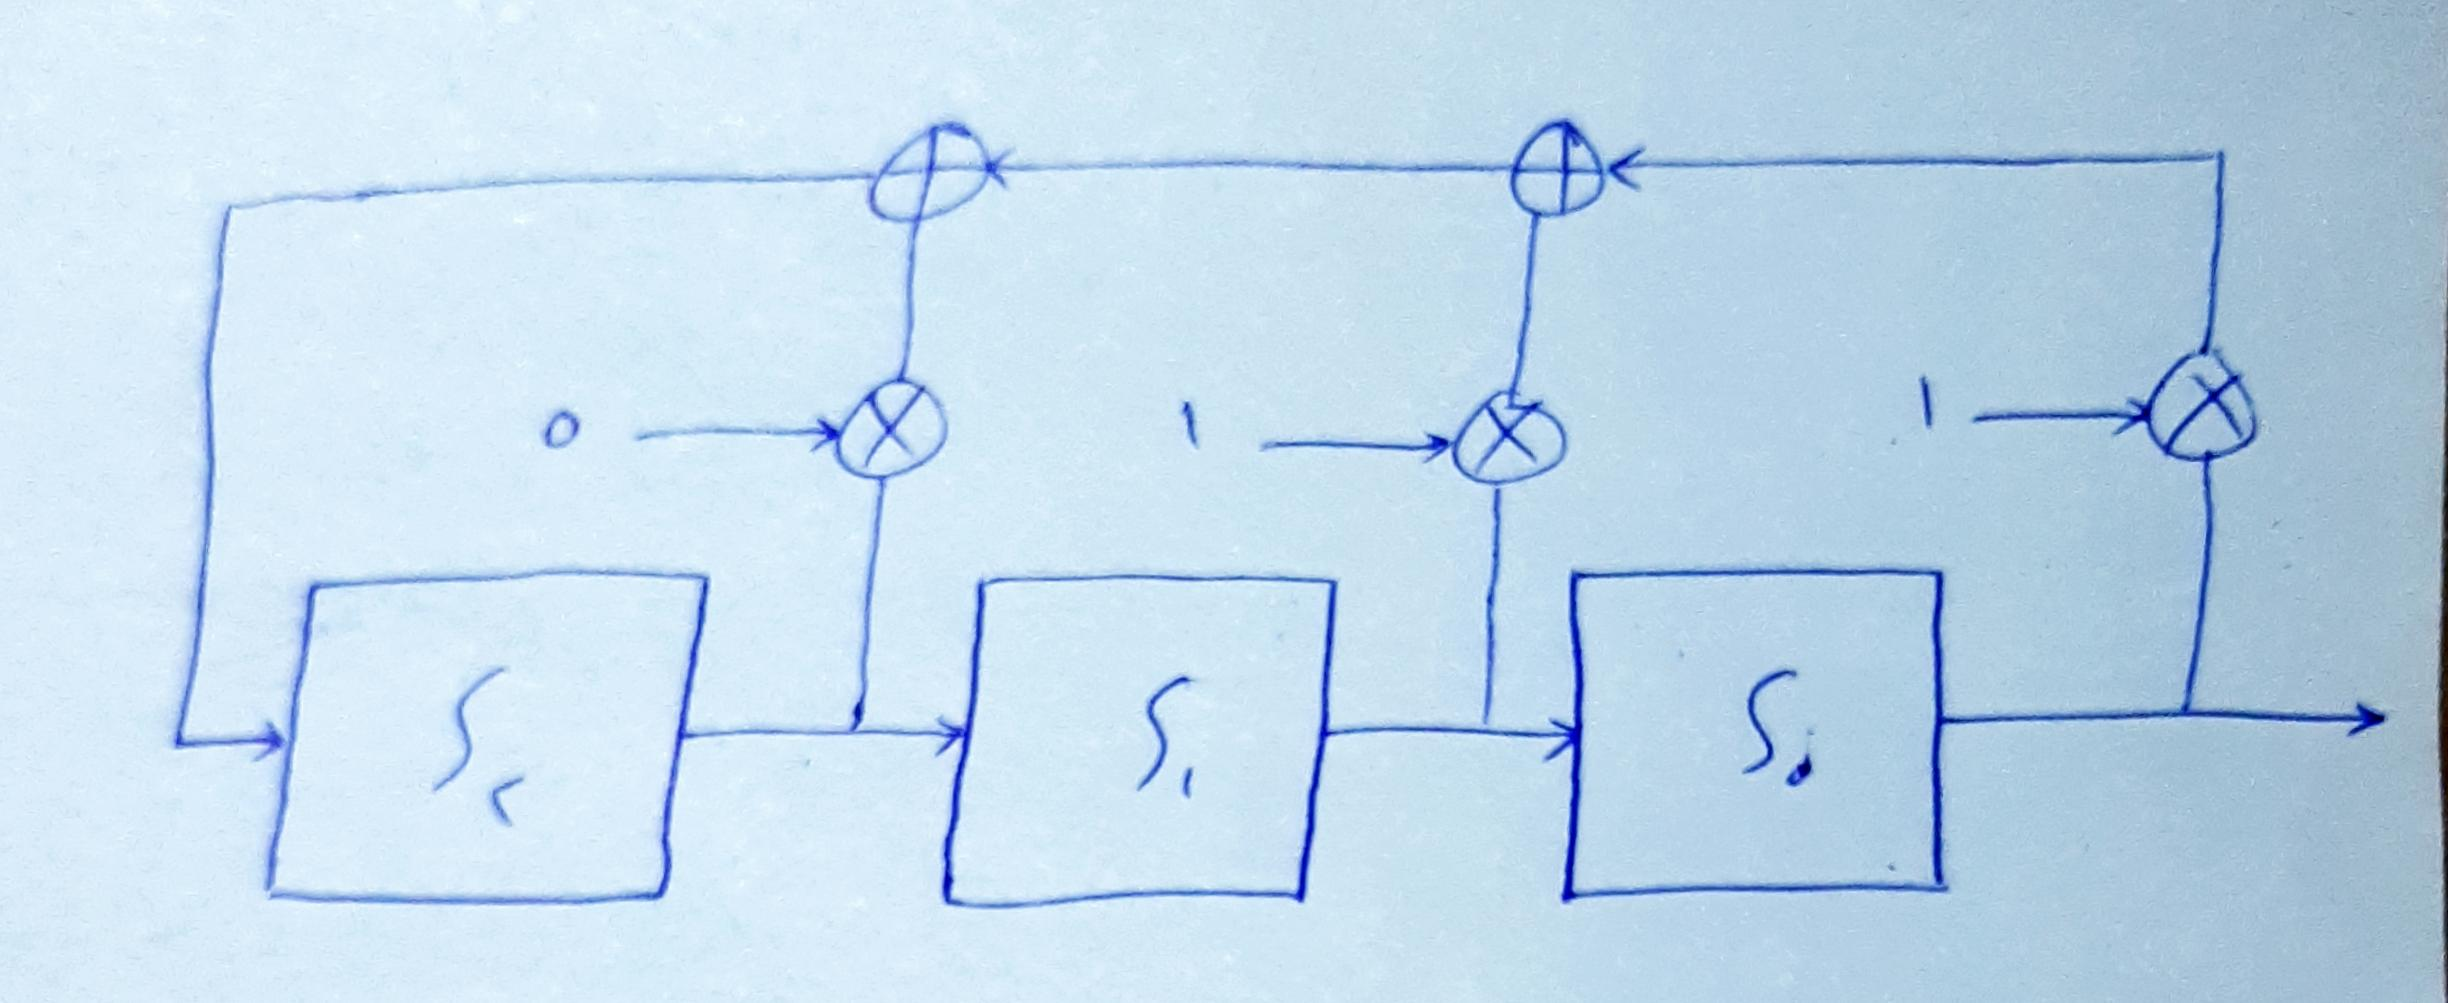
\includegraphics[width=0.75\textwidth]{figures/2.jpg}
    \caption
	{}
    \label{fig:fig1}
\end{figure}


%%%%%%%%%%%%%%%%%%%%%%%%%%%%%%%%%%%%%%%%%%
\section{\lr{CrypTool}}%2
\subsection{}
\subsubsection{\lr{a}}
کلید \lr{Caesar cipher} برابر \lr{M} است که حرف 13ام الفبای انگلیسی است. پس در واقع هر حرفِ الفبا به صورت حلقوی 12 واحد شیفت می‌خورد. پس در نهایت به صورت زیر رمز می‌شود.
\begin{latin}
% Please add the following required packages to your document preamble:
% \usepackage{graphicx}
\begin{table}[H]
\centering
\resizebox{\columnwidth}{!}{%
\begin{tabular}{|c|c|c|c|c|c|c|c|c|c|c|c|c|c|c|c|c|c|c|c|c|}
\hline
x           & A & l & i & r & e & z & a &  & A & b & r & e & h & f & o & r & o & u & s & h \\ \hline
$E_{12}(x)$ & M & x & u & d & q & l & m &  & M & n & d & q & t & r & a & d & a & g & e & t \\ \hline
\end{tabular}%
}
\end{table}
\end{latin}
در نرم افزار \lr{CrypTool} به صورت زیر رمز می‌کنیم.
\begin{figure}[H]
    \centering
    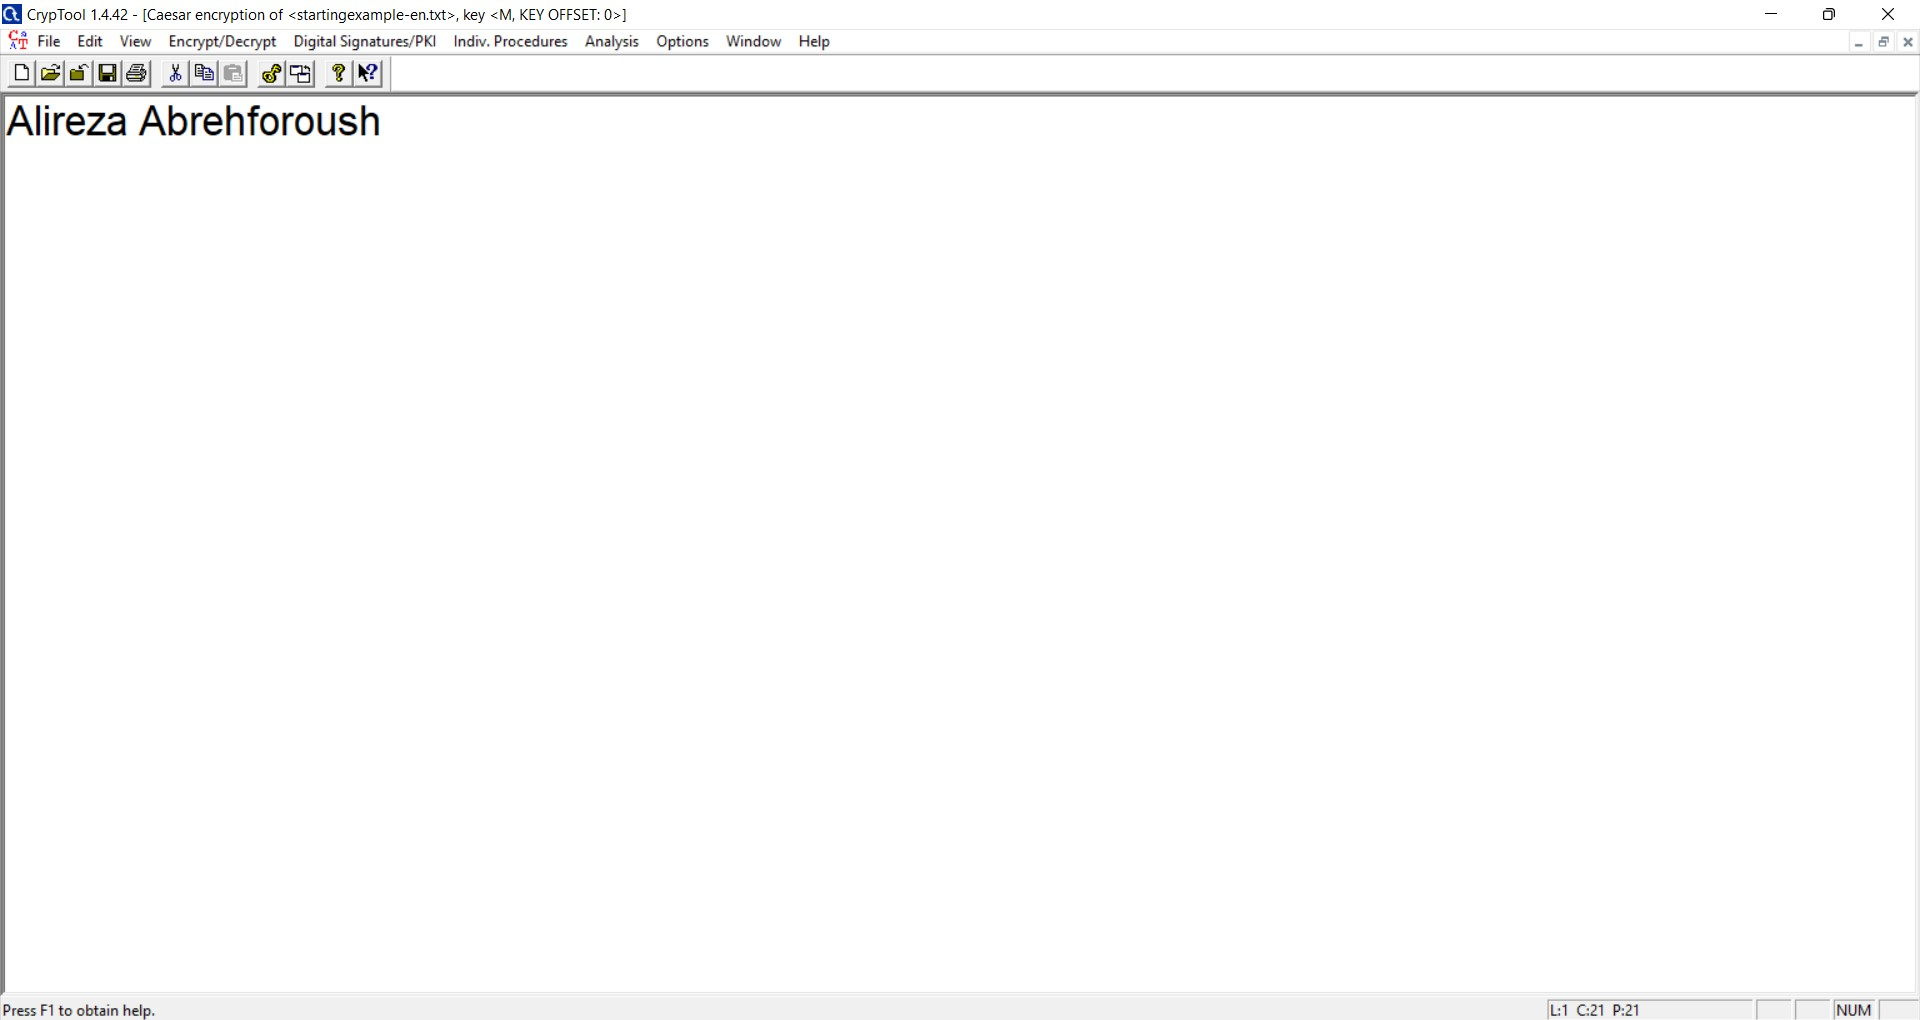
\includegraphics[width=0.75\textwidth]{figures/1a.jpg}
    \caption
	{}
    \label{fig:fig1}
\end{figure}

\begin{figure}[H]
    \centering
    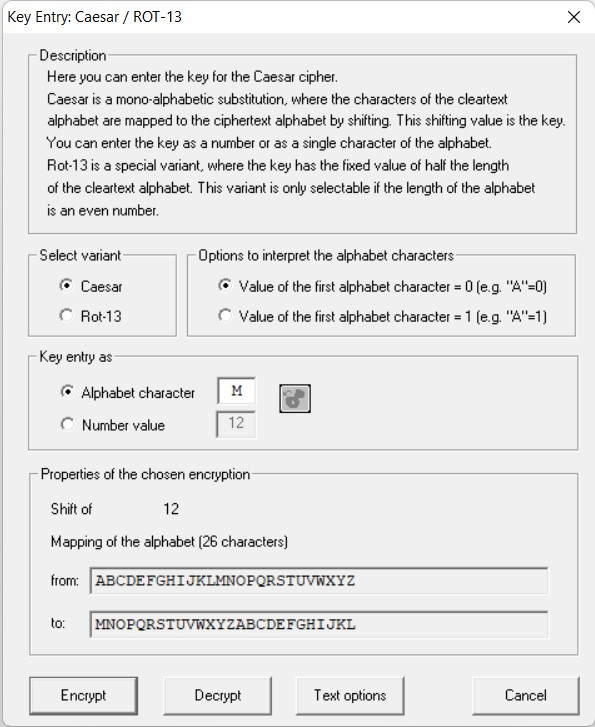
\includegraphics[width=0.75\textwidth]{figures/1b.jpg}
    \caption
	{}
    \label{fig:fig1}
\end{figure}

\begin{figure}[H]
    \centering
    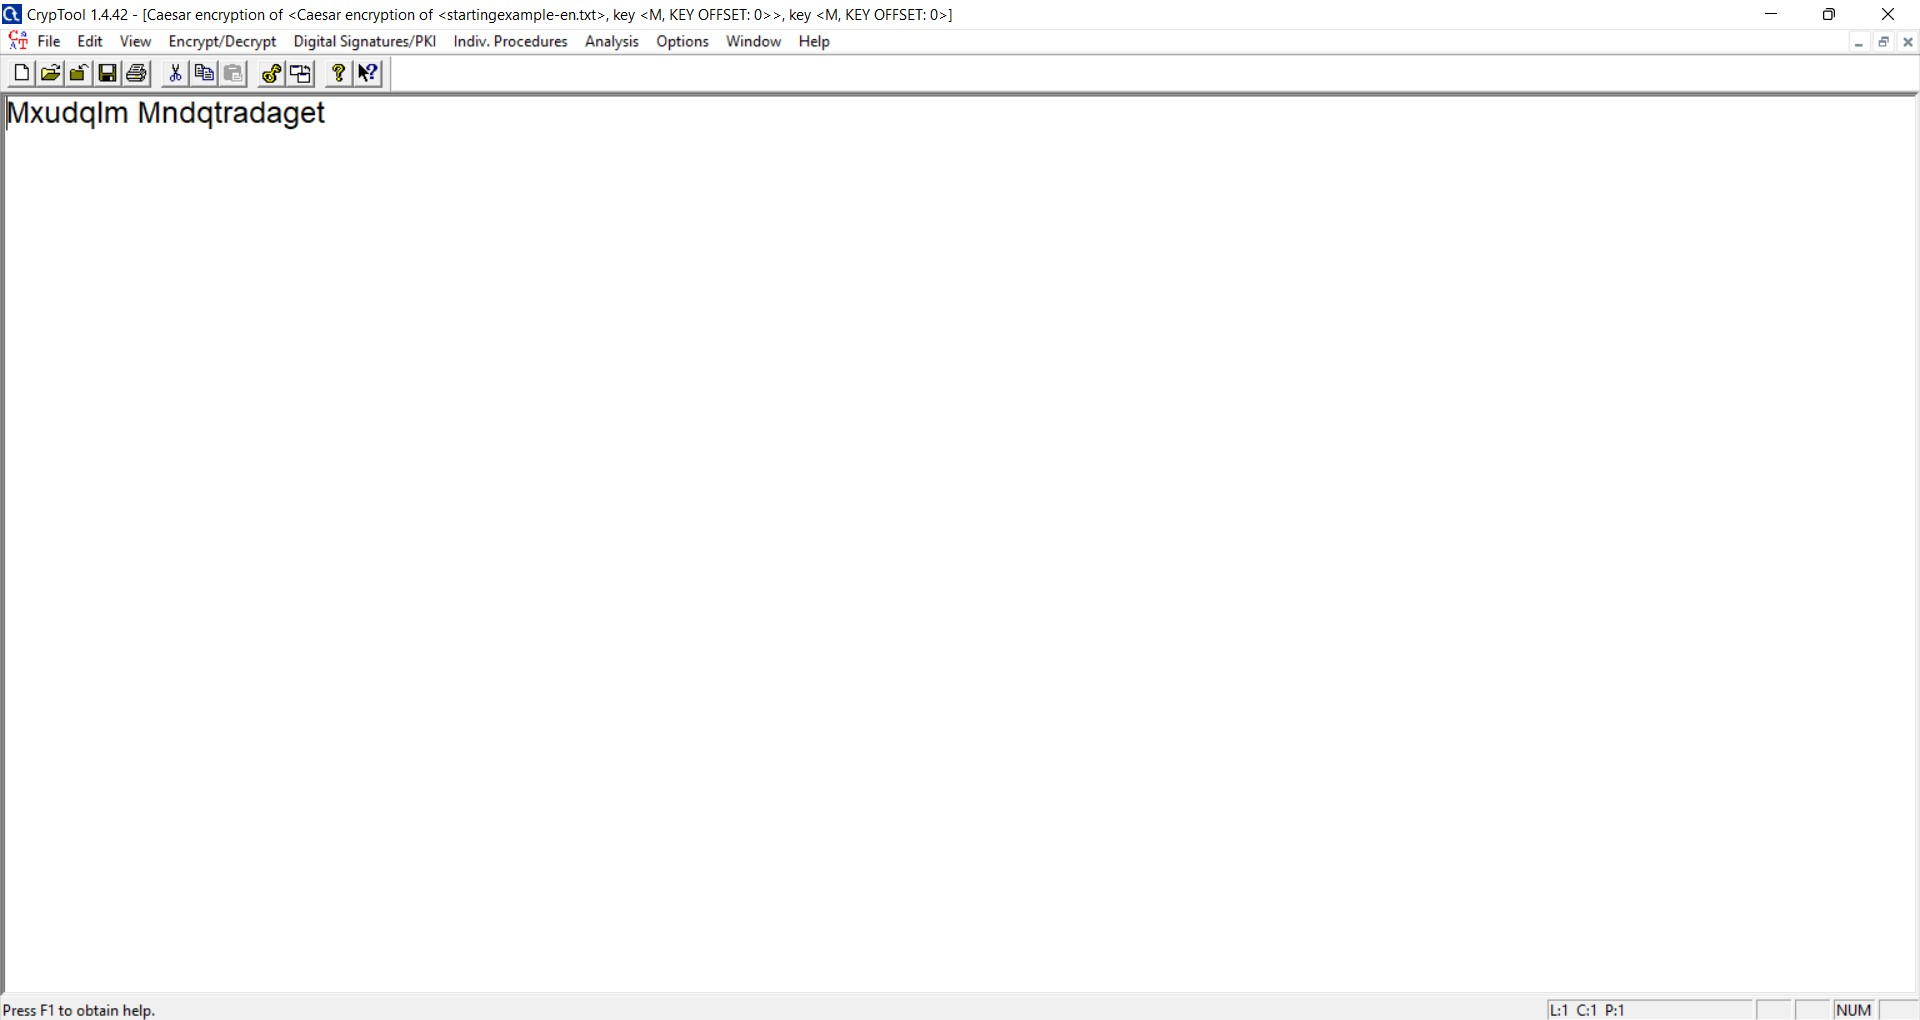
\includegraphics[width=0.75\textwidth]{figures/1c.jpg}
    \caption
	{}
    \label{fig:fig1}
\end{figure}

\subsection{}%2
\begin{latin}
$
9816603 \equiv 17 \:\:\:\:mod\:\: 26
$
\end{latin}
کلید \lr{Substitution cipher} برابر \lr{fharjolyinectzspdbkwxgumvq} و \lr{offset} آن برابر 17 است. در واقع الفبای انگلیسی به ترتیب به \lr{NECTZSPDBKWXGUMVQFHARJOLYI} \lr{map} می‌شود. پس در نهایت به صورت زیر رمز می‌شود.
\begin{latin}
% Please add the following required packages to your document preamble:
% \usepackage{graphicx}
\begin{table}[H]
\centering
\resizebox{\columnwidth}{!}{%
\begin{tabular}{|c|c|c|c|c|c|c|c|c|c|c|c|c|c|c|c|c|c|c|c|c|c|c|c|c|c|c|c|c|c|c|c|c|c|c|c|c|c|c|c|c|c|c|c|c|c|c|c|c|c|c|c|c|c|c|c|c|c|c|c|c|c|c|c|c|c|c|c|c|c|}
\hline
x           & S & u & c & c & e & s & s &  & u & s & u & a & l & l & y &  & c & o & m & e & s &  & t & o &  & t & h & o & s & e &  & w & h & o &  & a & r & e &  & t & o & o &  & b & u & s & y &  & t & o &  & b & e &  & l & o & o & k & i & n & g &  & f & o & r &  & i & t & . \\ \hline
$E(x)$ & H & r & c & c & z & h & h &  & r & h & r & n & x & x & y &  & c & m & g & z & h &  & a & m &  & a & d & m & h & z &  & o & d & m &  & n & f & z &  & a & m & m &  & e & r & h & y &  & a & m &  & e & z &  & x & m & m & w & b & u & p &  & s & m & f &  & b & a & . \\ \hline
\end{tabular}%
}
\end{table}
\end{latin}
در نرم افزار \lr{CrypTool} به صورت زیر رمز می‌کنیم.
\begin{figure}[H]
    \centering
    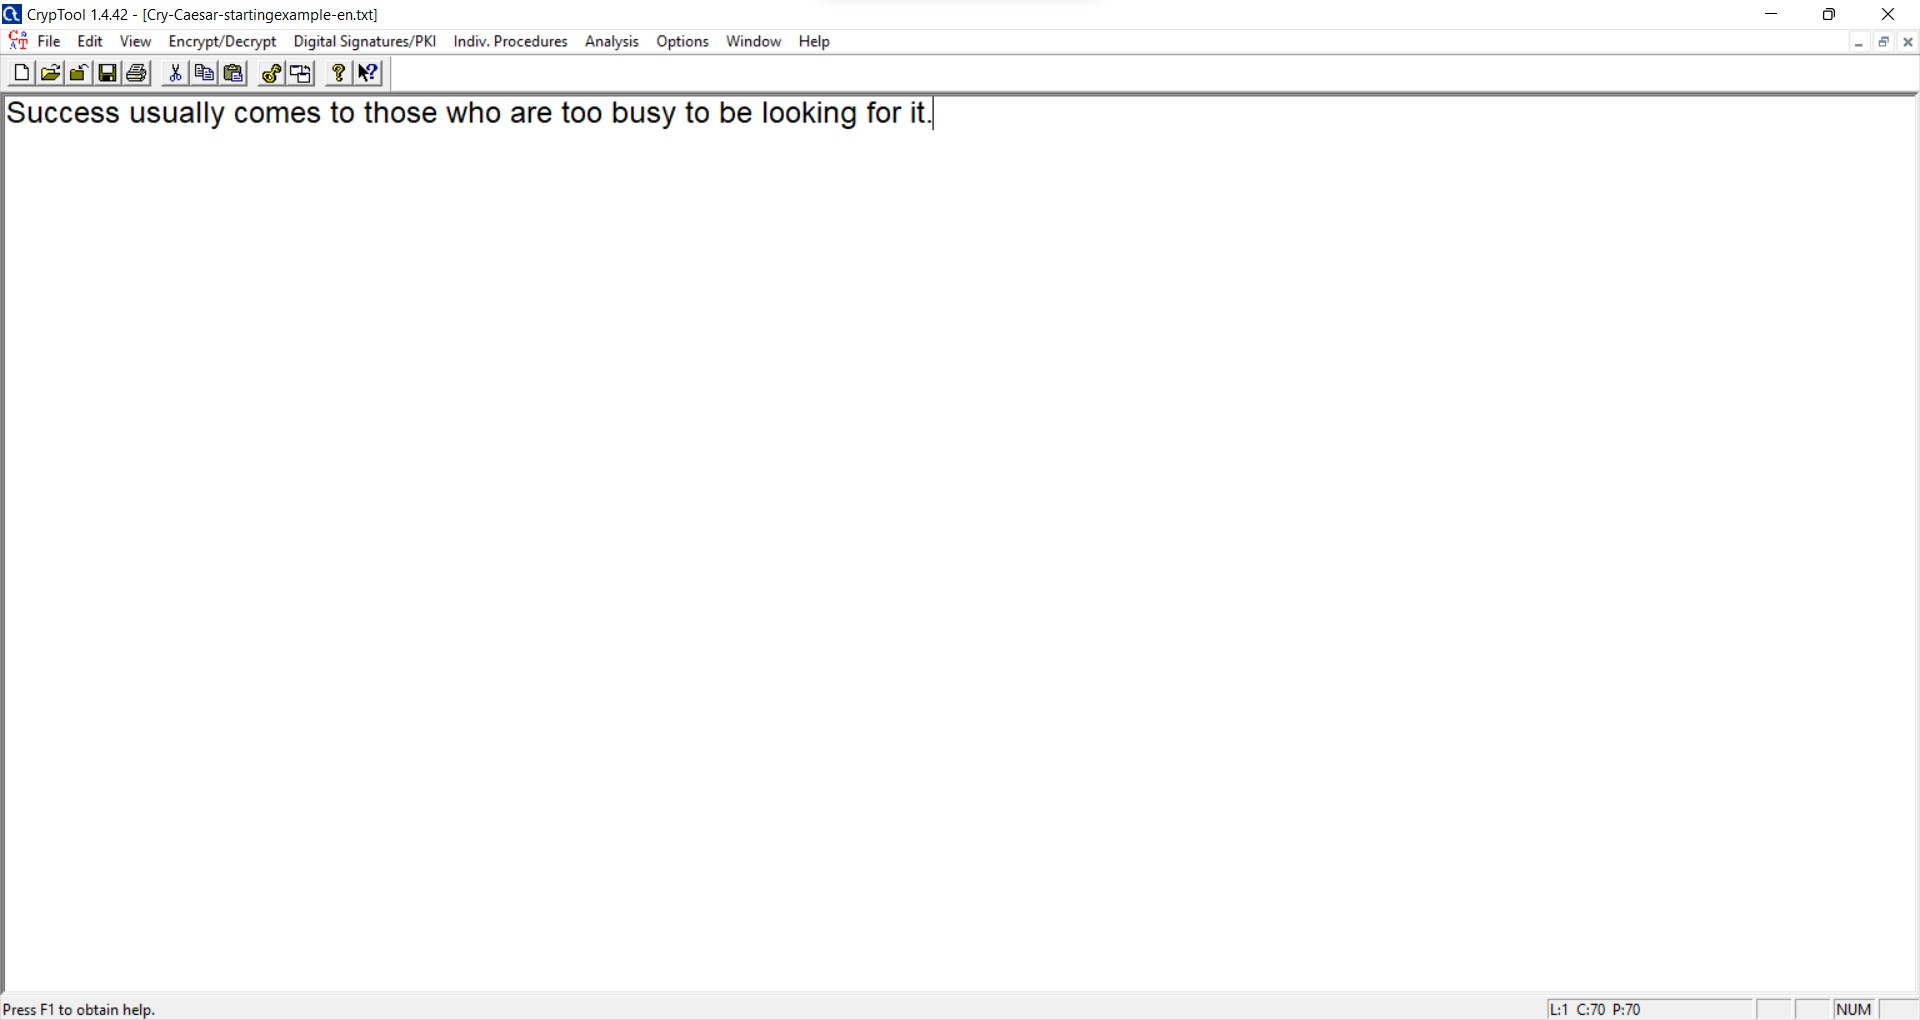
\includegraphics[width=0.75\textwidth]{figures/2a.jpg}
    \caption
	{}
    \label{fig:fig1}
\end{figure}

\begin{figure}[H]
    \centering
    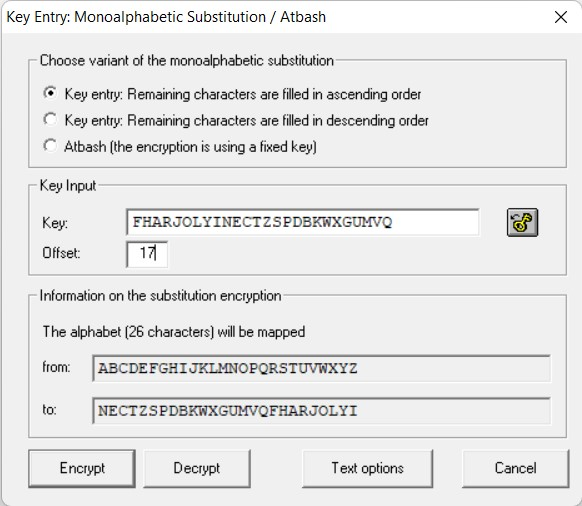
\includegraphics[width=0.75\textwidth]{figures/2b.jpg}
    \caption
	{}
    \label{fig:fig1}
\end{figure}

\begin{figure}[H]
    \centering
    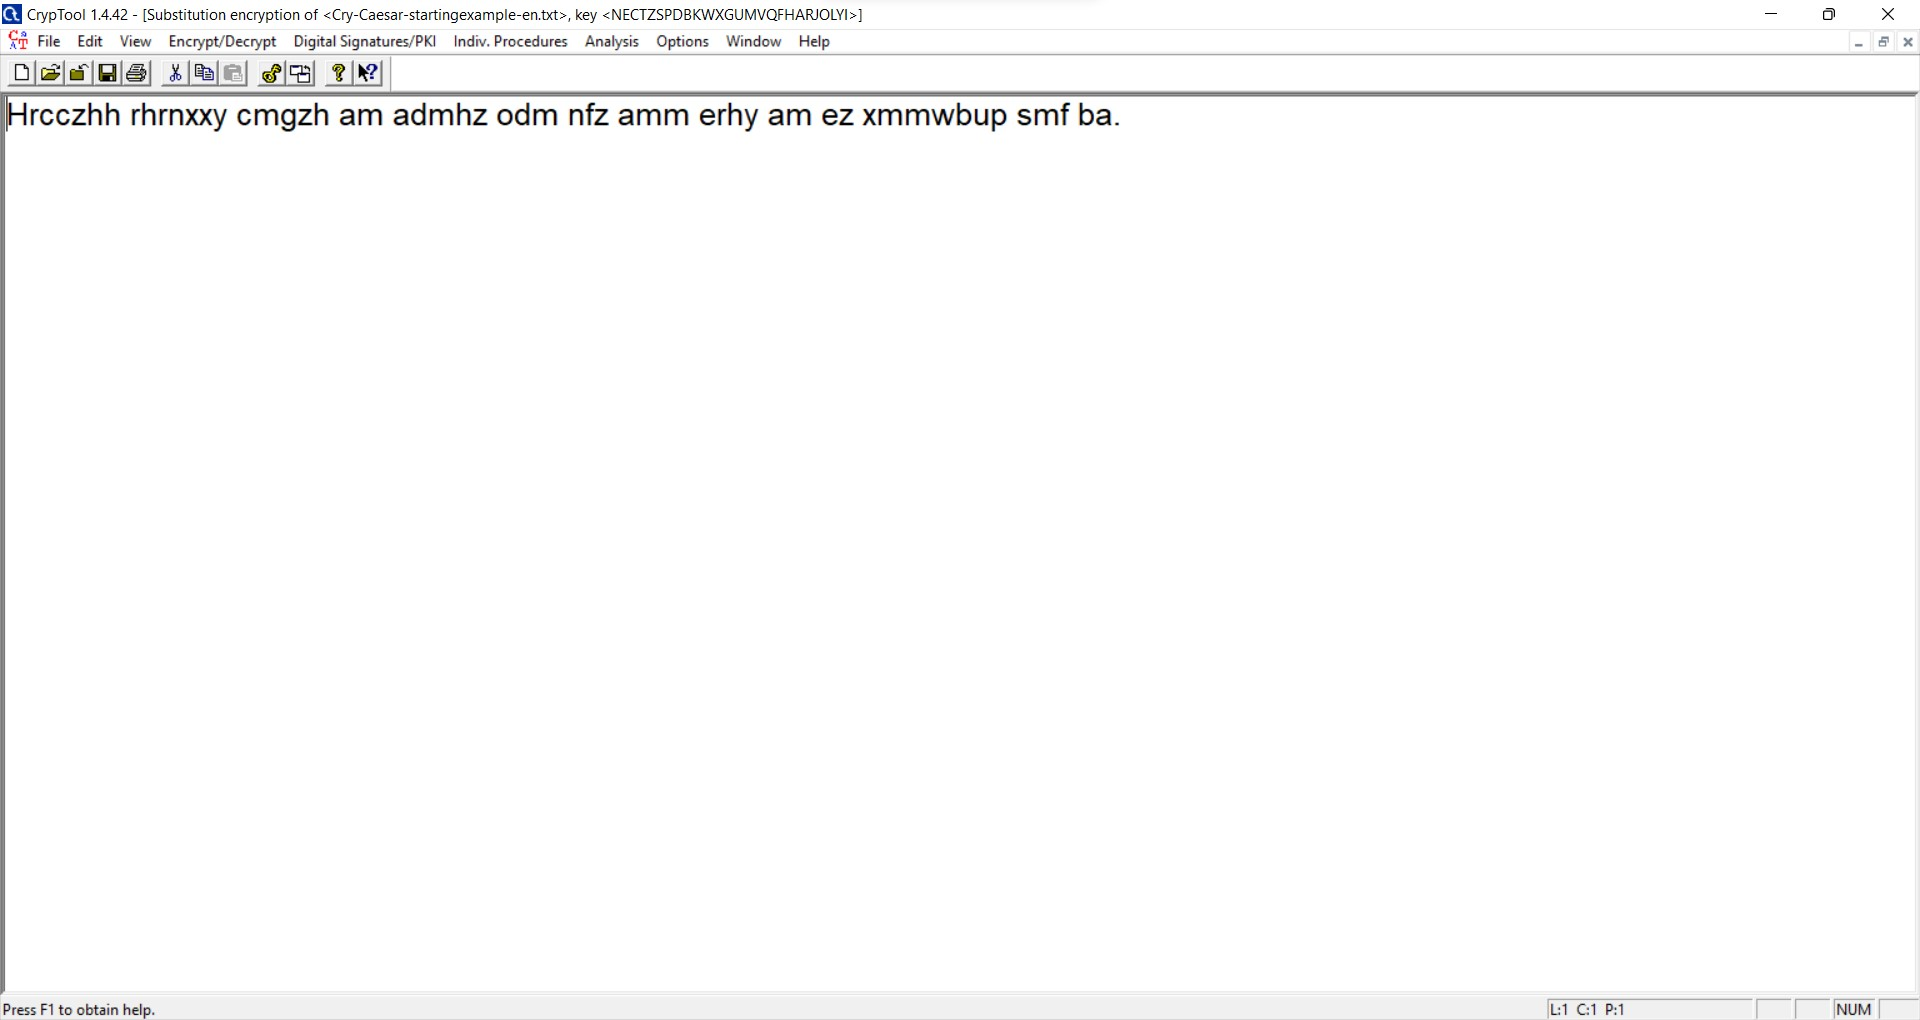
\includegraphics[width=0.75\textwidth]{figures/2c.jpg}
    \caption
	{}
    \label{fig:fig1}
\end{figure}


\subsection{}%3
\subsubsection{\lr{a}}
در \lr{Vigenère cipher} در الفبای انگلیسی از یک جدول با ابعاد $26 \times 26$ استفاده می‌شود که در سطر $i$ام آن حروف انگلیسی به ترتیب به صورت حلقوی با شروع از حرف $i$ام الفبا نوشته شده است.
\begin{latin}
% Please add the following required packages to your document preamble:
% \usepackage{graphicx}
\begin{table}[H]
\centering
\resizebox{\columnwidth}{!}{%
\begin{tabular}{ccccccccccccccccccccccccccc}
                                & \textbf{A}             & \textbf{B}             & \textbf{C}             & \textbf{D}             & \textbf{E}             & \textbf{F}             & \textbf{G}             & \textbf{H}             & \textbf{I}             & \textbf{J}             & \textbf{K}             & \textbf{L}             & \textbf{M}             & \textbf{N}             & \textbf{O}             & \textbf{P}             & \textbf{Q}             & \textbf{R}             & \textbf{S}             & \textbf{T}             & \textbf{U}             & \textbf{V}             & \textbf{W}             & \textbf{X}             & \textbf{Y}             & \textbf{Z}             \\ \cline{2-27} 
\multicolumn{1}{c|}{\textbf{A}} & \multicolumn{1}{c|}{A} & \multicolumn{1}{c|}{B} & \multicolumn{1}{c|}{C} & \multicolumn{1}{c|}{D} & \multicolumn{1}{c|}{E} & \multicolumn{1}{c|}{F} & \multicolumn{1}{c|}{G} & \multicolumn{1}{c|}{H} & \multicolumn{1}{c|}{I} & \multicolumn{1}{c|}{J} & \multicolumn{1}{c|}{K} & \multicolumn{1}{c|}{L} & \multicolumn{1}{c|}{M} & \multicolumn{1}{c|}{N} & \multicolumn{1}{c|}{O} & \multicolumn{1}{c|}{P} & \multicolumn{1}{c|}{Q} & \multicolumn{1}{c|}{R} & \multicolumn{1}{c|}{S} & \multicolumn{1}{c|}{T} & \multicolumn{1}{c|}{U} & \multicolumn{1}{c|}{V} & \multicolumn{1}{c|}{W} & \multicolumn{1}{c|}{X} & \multicolumn{1}{c|}{Y} & \multicolumn{1}{c|}{Z} \\ \cline{2-27} 
\multicolumn{1}{c|}{\textbf{B}} & \multicolumn{1}{c|}{B} & \multicolumn{1}{c|}{C} & \multicolumn{1}{c|}{D} & \multicolumn{1}{c|}{E} & \multicolumn{1}{c|}{F} & \multicolumn{1}{c|}{G} & \multicolumn{1}{c|}{H} & \multicolumn{1}{c|}{I} & \multicolumn{1}{c|}{J} & \multicolumn{1}{c|}{K} & \multicolumn{1}{c|}{L} & \multicolumn{1}{c|}{M} & \multicolumn{1}{c|}{N} & \multicolumn{1}{c|}{O} & \multicolumn{1}{c|}{P} & \multicolumn{1}{c|}{Q} & \multicolumn{1}{c|}{R} & \multicolumn{1}{c|}{S} & \multicolumn{1}{c|}{T} & \multicolumn{1}{c|}{U} & \multicolumn{1}{c|}{V} & \multicolumn{1}{c|}{W} & \multicolumn{1}{c|}{X} & \multicolumn{1}{c|}{Y} & \multicolumn{1}{c|}{Z} & \multicolumn{1}{c|}{A} \\ \cline{2-27} 
\multicolumn{1}{c|}{\textbf{C}} & \multicolumn{1}{c|}{C} & \multicolumn{1}{c|}{D} & \multicolumn{1}{c|}{E} & \multicolumn{1}{c|}{F} & \multicolumn{1}{c|}{G} & \multicolumn{1}{c|}{H} & \multicolumn{1}{c|}{I} & \multicolumn{1}{c|}{J} & \multicolumn{1}{c|}{K} & \multicolumn{1}{c|}{L} & \multicolumn{1}{c|}{M} & \multicolumn{1}{c|}{N} & \multicolumn{1}{c|}{O} & \multicolumn{1}{c|}{P} & \multicolumn{1}{c|}{Q} & \multicolumn{1}{c|}{R} & \multicolumn{1}{c|}{S} & \multicolumn{1}{c|}{T} & \multicolumn{1}{c|}{U} & \multicolumn{1}{c|}{V} & \multicolumn{1}{c|}{W} & \multicolumn{1}{c|}{X} & \multicolumn{1}{c|}{Y} & \multicolumn{1}{c|}{Z} & \multicolumn{1}{c|}{A} & \multicolumn{1}{c|}{B} \\ \cline{2-27} 
\multicolumn{1}{c|}{\textbf{D}} & \multicolumn{1}{c|}{D} & \multicolumn{1}{c|}{E} & \multicolumn{1}{c|}{F} & \multicolumn{1}{c|}{G} & \multicolumn{1}{c|}{H} & \multicolumn{1}{c|}{I} & \multicolumn{1}{c|}{J} & \multicolumn{1}{c|}{K} & \multicolumn{1}{c|}{L} & \multicolumn{1}{c|}{M} & \multicolumn{1}{c|}{N} & \multicolumn{1}{c|}{O} & \multicolumn{1}{c|}{P} & \multicolumn{1}{c|}{Q} & \multicolumn{1}{c|}{R} & \multicolumn{1}{c|}{S} & \multicolumn{1}{c|}{T} & \multicolumn{1}{c|}{U} & \multicolumn{1}{c|}{V} & \multicolumn{1}{c|}{W} & \multicolumn{1}{c|}{X} & \multicolumn{1}{c|}{Y} & \multicolumn{1}{c|}{Z} & \multicolumn{1}{c|}{A} & \multicolumn{1}{c|}{B} & \multicolumn{1}{c|}{C} \\ \cline{2-27} 
\multicolumn{1}{c|}{\textbf{E}} & \multicolumn{1}{c|}{E} & \multicolumn{1}{c|}{F} & \multicolumn{1}{c|}{G} & \multicolumn{1}{c|}{H} & \multicolumn{1}{c|}{I} & \multicolumn{1}{c|}{J} & \multicolumn{1}{c|}{K} & \multicolumn{1}{c|}{L} & \multicolumn{1}{c|}{M} & \multicolumn{1}{c|}{N} & \multicolumn{1}{c|}{O} & \multicolumn{1}{c|}{P} & \multicolumn{1}{c|}{Q} & \multicolumn{1}{c|}{R} & \multicolumn{1}{c|}{S} & \multicolumn{1}{c|}{T} & \multicolumn{1}{c|}{U} & \multicolumn{1}{c|}{V} & \multicolumn{1}{c|}{W} & \multicolumn{1}{c|}{X} & \multicolumn{1}{c|}{Y} & \multicolumn{1}{c|}{Z} & \multicolumn{1}{c|}{A} & \multicolumn{1}{c|}{B} & \multicolumn{1}{c|}{C} & \multicolumn{1}{c|}{D} \\ \cline{2-27} 
\multicolumn{1}{c|}{\textbf{F}} & \multicolumn{1}{c|}{F} & \multicolumn{1}{c|}{G} & \multicolumn{1}{c|}{H} & \multicolumn{1}{c|}{I} & \multicolumn{1}{c|}{J} & \multicolumn{1}{c|}{K} & \multicolumn{1}{c|}{L} & \multicolumn{1}{c|}{M} & \multicolumn{1}{c|}{N} & \multicolumn{1}{c|}{O} & \multicolumn{1}{c|}{P} & \multicolumn{1}{c|}{Q} & \multicolumn{1}{c|}{R} & \multicolumn{1}{c|}{S} & \multicolumn{1}{c|}{T} & \multicolumn{1}{c|}{U} & \multicolumn{1}{c|}{V} & \multicolumn{1}{c|}{W} & \multicolumn{1}{c|}{X} & \multicolumn{1}{c|}{Y} & \multicolumn{1}{c|}{Z} & \multicolumn{1}{c|}{A} & \multicolumn{1}{c|}{B} & \multicolumn{1}{c|}{C} & \multicolumn{1}{c|}{D} & \multicolumn{1}{c|}{E} \\ \cline{2-27} 
\multicolumn{1}{c|}{\textbf{G}} & \multicolumn{1}{c|}{G} & \multicolumn{1}{c|}{H} & \multicolumn{1}{c|}{I} & \multicolumn{1}{c|}{J} & \multicolumn{1}{c|}{K} & \multicolumn{1}{c|}{L} & \multicolumn{1}{c|}{M} & \multicolumn{1}{c|}{N} & \multicolumn{1}{c|}{O} & \multicolumn{1}{c|}{P} & \multicolumn{1}{c|}{Q} & \multicolumn{1}{c|}{R} & \multicolumn{1}{c|}{S} & \multicolumn{1}{c|}{T} & \multicolumn{1}{c|}{U} & \multicolumn{1}{c|}{V} & \multicolumn{1}{c|}{W} & \multicolumn{1}{c|}{X} & \multicolumn{1}{c|}{Y} & \multicolumn{1}{c|}{Z} & \multicolumn{1}{c|}{A} & \multicolumn{1}{c|}{B} & \multicolumn{1}{c|}{C} & \multicolumn{1}{c|}{D} & \multicolumn{1}{c|}{E} & \multicolumn{1}{c|}{F} \\ \cline{2-27} 
\multicolumn{1}{c|}{\textbf{H}} & \multicolumn{1}{c|}{H} & \multicolumn{1}{c|}{I} & \multicolumn{1}{c|}{J} & \multicolumn{1}{c|}{K} & \multicolumn{1}{c|}{L} & \multicolumn{1}{c|}{M} & \multicolumn{1}{c|}{N} & \multicolumn{1}{c|}{O} & \multicolumn{1}{c|}{P} & \multicolumn{1}{c|}{Q} & \multicolumn{1}{c|}{R} & \multicolumn{1}{c|}{S} & \multicolumn{1}{c|}{T} & \multicolumn{1}{c|}{U} & \multicolumn{1}{c|}{V} & \multicolumn{1}{c|}{W} & \multicolumn{1}{c|}{X} & \multicolumn{1}{c|}{Y} & \multicolumn{1}{c|}{Z} & \multicolumn{1}{c|}{A} & \multicolumn{1}{c|}{B} & \multicolumn{1}{c|}{C} & \multicolumn{1}{c|}{D} & \multicolumn{1}{c|}{E} & \multicolumn{1}{c|}{F} & \multicolumn{1}{c|}{G} \\ \cline{2-27} 
\multicolumn{1}{c|}{\textbf{I}} & \multicolumn{1}{c|}{I} & \multicolumn{1}{c|}{J} & \multicolumn{1}{c|}{K} & \multicolumn{1}{c|}{L} & \multicolumn{1}{c|}{M} & \multicolumn{1}{c|}{N} & \multicolumn{1}{c|}{O} & \multicolumn{1}{c|}{P} & \multicolumn{1}{c|}{Q} & \multicolumn{1}{c|}{R} & \multicolumn{1}{c|}{S} & \multicolumn{1}{c|}{T} & \multicolumn{1}{c|}{U} & \multicolumn{1}{c|}{V} & \multicolumn{1}{c|}{W} & \multicolumn{1}{c|}{X} & \multicolumn{1}{c|}{Y} & \multicolumn{1}{c|}{Z} & \multicolumn{1}{c|}{A} & \multicolumn{1}{c|}{B} & \multicolumn{1}{c|}{C} & \multicolumn{1}{c|}{D} & \multicolumn{1}{c|}{E} & \multicolumn{1}{c|}{F} & \multicolumn{1}{c|}{G} & \multicolumn{1}{c|}{H} \\ \cline{2-27} 
\multicolumn{1}{c|}{\textbf{J}} & \multicolumn{1}{c|}{J} & \multicolumn{1}{c|}{K} & \multicolumn{1}{c|}{L} & \multicolumn{1}{c|}{M} & \multicolumn{1}{c|}{N} & \multicolumn{1}{c|}{O} & \multicolumn{1}{c|}{P} & \multicolumn{1}{c|}{Q} & \multicolumn{1}{c|}{R} & \multicolumn{1}{c|}{S} & \multicolumn{1}{c|}{T} & \multicolumn{1}{c|}{U} & \multicolumn{1}{c|}{V} & \multicolumn{1}{c|}{W} & \multicolumn{1}{c|}{X} & \multicolumn{1}{c|}{Y} & \multicolumn{1}{c|}{Z} & \multicolumn{1}{c|}{A} & \multicolumn{1}{c|}{B} & \multicolumn{1}{c|}{C} & \multicolumn{1}{c|}{D} & \multicolumn{1}{c|}{E} & \multicolumn{1}{c|}{F} & \multicolumn{1}{c|}{G} & \multicolumn{1}{c|}{H} & \multicolumn{1}{c|}{I} \\ \cline{2-27} 
\multicolumn{1}{c|}{\textbf{K}} & \multicolumn{1}{c|}{K} & \multicolumn{1}{c|}{L} & \multicolumn{1}{c|}{M} & \multicolumn{1}{c|}{N} & \multicolumn{1}{c|}{O} & \multicolumn{1}{c|}{P} & \multicolumn{1}{c|}{Q} & \multicolumn{1}{c|}{R} & \multicolumn{1}{c|}{S} & \multicolumn{1}{c|}{T} & \multicolumn{1}{c|}{U} & \multicolumn{1}{c|}{V} & \multicolumn{1}{c|}{W} & \multicolumn{1}{c|}{X} & \multicolumn{1}{c|}{Y} & \multicolumn{1}{c|}{Z} & \multicolumn{1}{c|}{A} & \multicolumn{1}{c|}{B} & \multicolumn{1}{c|}{C} & \multicolumn{1}{c|}{D} & \multicolumn{1}{c|}{E} & \multicolumn{1}{c|}{F} & \multicolumn{1}{c|}{G} & \multicolumn{1}{c|}{H} & \multicolumn{1}{c|}{I} & \multicolumn{1}{c|}{J} \\ \cline{2-27} 
\multicolumn{1}{c|}{\textbf{L}} & \multicolumn{1}{c|}{L} & \multicolumn{1}{c|}{M} & \multicolumn{1}{c|}{N} & \multicolumn{1}{c|}{O} & \multicolumn{1}{c|}{P} & \multicolumn{1}{c|}{Q} & \multicolumn{1}{c|}{R} & \multicolumn{1}{c|}{S} & \multicolumn{1}{c|}{T} & \multicolumn{1}{c|}{U} & \multicolumn{1}{c|}{V} & \multicolumn{1}{c|}{W} & \multicolumn{1}{c|}{X} & \multicolumn{1}{c|}{Y} & \multicolumn{1}{c|}{Z} & \multicolumn{1}{c|}{A} & \multicolumn{1}{c|}{B} & \multicolumn{1}{c|}{C} & \multicolumn{1}{c|}{D} & \multicolumn{1}{c|}{E} & \multicolumn{1}{c|}{F} & \multicolumn{1}{c|}{G} & \multicolumn{1}{c|}{H} & \multicolumn{1}{c|}{I} & \multicolumn{1}{c|}{J} & \multicolumn{1}{c|}{K} \\ \cline{2-27} 
\multicolumn{1}{c|}{\textbf{M}} & \multicolumn{1}{c|}{M} & \multicolumn{1}{c|}{N} & \multicolumn{1}{c|}{O} & \multicolumn{1}{c|}{P} & \multicolumn{1}{c|}{Q} & \multicolumn{1}{c|}{R} & \multicolumn{1}{c|}{S} & \multicolumn{1}{c|}{T} & \multicolumn{1}{c|}{U} & \multicolumn{1}{c|}{V} & \multicolumn{1}{c|}{W} & \multicolumn{1}{c|}{X} & \multicolumn{1}{c|}{Y} & \multicolumn{1}{c|}{Z} & \multicolumn{1}{c|}{A} & \multicolumn{1}{c|}{B} & \multicolumn{1}{c|}{C} & \multicolumn{1}{c|}{D} & \multicolumn{1}{c|}{E} & \multicolumn{1}{c|}{F} & \multicolumn{1}{c|}{G} & \multicolumn{1}{c|}{H} & \multicolumn{1}{c|}{I} & \multicolumn{1}{c|}{J} & \multicolumn{1}{c|}{K} & \multicolumn{1}{c|}{L} \\ \cline{2-27} 
\multicolumn{1}{c|}{\textbf{N}} & \multicolumn{1}{c|}{N} & \multicolumn{1}{c|}{O} & \multicolumn{1}{c|}{P} & \multicolumn{1}{c|}{Q} & \multicolumn{1}{c|}{R} & \multicolumn{1}{c|}{S} & \multicolumn{1}{c|}{T} & \multicolumn{1}{c|}{U} & \multicolumn{1}{c|}{V} & \multicolumn{1}{c|}{W} & \multicolumn{1}{c|}{X} & \multicolumn{1}{c|}{Y} & \multicolumn{1}{c|}{Z} & \multicolumn{1}{c|}{A} & \multicolumn{1}{c|}{B} & \multicolumn{1}{c|}{C} & \multicolumn{1}{c|}{D} & \multicolumn{1}{c|}{E} & \multicolumn{1}{c|}{F} & \multicolumn{1}{c|}{G} & \multicolumn{1}{c|}{H} & \multicolumn{1}{c|}{I} & \multicolumn{1}{c|}{J} & \multicolumn{1}{c|}{K} & \multicolumn{1}{c|}{L} & \multicolumn{1}{c|}{M} \\ \cline{2-27} 
\multicolumn{1}{c|}{\textbf{O}} & \multicolumn{1}{c|}{O} & \multicolumn{1}{c|}{P} & \multicolumn{1}{c|}{Q} & \multicolumn{1}{c|}{R} & \multicolumn{1}{c|}{S} & \multicolumn{1}{c|}{T} & \multicolumn{1}{c|}{U} & \multicolumn{1}{c|}{V} & \multicolumn{1}{c|}{W} & \multicolumn{1}{c|}{X} & \multicolumn{1}{c|}{Y} & \multicolumn{1}{c|}{Z} & \multicolumn{1}{c|}{A} & \multicolumn{1}{c|}{B} & \multicolumn{1}{c|}{C} & \multicolumn{1}{c|}{D} & \multicolumn{1}{c|}{E} & \multicolumn{1}{c|}{F} & \multicolumn{1}{c|}{G} & \multicolumn{1}{c|}{H} & \multicolumn{1}{c|}{I} & \multicolumn{1}{c|}{J} & \multicolumn{1}{c|}{K} & \multicolumn{1}{c|}{L} & \multicolumn{1}{c|}{M} & \multicolumn{1}{c|}{N} \\ \cline{2-27} 
\multicolumn{1}{c|}{\textbf{P}} & \multicolumn{1}{c|}{P} & \multicolumn{1}{c|}{Q} & \multicolumn{1}{c|}{R} & \multicolumn{1}{c|}{S} & \multicolumn{1}{c|}{T} & \multicolumn{1}{c|}{U} & \multicolumn{1}{c|}{V} & \multicolumn{1}{c|}{W} & \multicolumn{1}{c|}{X} & \multicolumn{1}{c|}{Y} & \multicolumn{1}{c|}{Z} & \multicolumn{1}{c|}{A} & \multicolumn{1}{c|}{B} & \multicolumn{1}{c|}{C} & \multicolumn{1}{c|}{D} & \multicolumn{1}{c|}{E} & \multicolumn{1}{c|}{F} & \multicolumn{1}{c|}{G} & \multicolumn{1}{c|}{H} & \multicolumn{1}{c|}{I} & \multicolumn{1}{c|}{J} & \multicolumn{1}{c|}{K} & \multicolumn{1}{c|}{L} & \multicolumn{1}{c|}{M} & \multicolumn{1}{c|}{N} & \multicolumn{1}{c|}{O} \\ \cline{2-27} 
\multicolumn{1}{c|}{\textbf{Q}} & \multicolumn{1}{c|}{Q} & \multicolumn{1}{c|}{R} & \multicolumn{1}{c|}{S} & \multicolumn{1}{c|}{T} & \multicolumn{1}{c|}{U} & \multicolumn{1}{c|}{V} & \multicolumn{1}{c|}{W} & \multicolumn{1}{c|}{X} & \multicolumn{1}{c|}{Y} & \multicolumn{1}{c|}{Z} & \multicolumn{1}{c|}{A} & \multicolumn{1}{c|}{B} & \multicolumn{1}{c|}{C} & \multicolumn{1}{c|}{D} & \multicolumn{1}{c|}{E} & \multicolumn{1}{c|}{F} & \multicolumn{1}{c|}{G} & \multicolumn{1}{c|}{H} & \multicolumn{1}{c|}{I} & \multicolumn{1}{c|}{J} & \multicolumn{1}{c|}{K} & \multicolumn{1}{c|}{L} & \multicolumn{1}{c|}{M} & \multicolumn{1}{c|}{N} & \multicolumn{1}{c|}{O} & \multicolumn{1}{c|}{P} \\ \cline{2-27} 
\multicolumn{1}{c|}{\textbf{R}} & \multicolumn{1}{c|}{R} & \multicolumn{1}{c|}{S} & \multicolumn{1}{c|}{T} & \multicolumn{1}{c|}{U} & \multicolumn{1}{c|}{V} & \multicolumn{1}{c|}{W} & \multicolumn{1}{c|}{X} & \multicolumn{1}{c|}{Y} & \multicolumn{1}{c|}{Z} & \multicolumn{1}{c|}{A} & \multicolumn{1}{c|}{B} & \multicolumn{1}{c|}{C} & \multicolumn{1}{c|}{D} & \multicolumn{1}{c|}{E} & \multicolumn{1}{c|}{F} & \multicolumn{1}{c|}{G} & \multicolumn{1}{c|}{H} & \multicolumn{1}{c|}{I} & \multicolumn{1}{c|}{J} & \multicolumn{1}{c|}{K} & \multicolumn{1}{c|}{L} & \multicolumn{1}{c|}{M} & \multicolumn{1}{c|}{N} & \multicolumn{1}{c|}{O} & \multicolumn{1}{c|}{P} & \multicolumn{1}{c|}{Q} \\ \cline{2-27} 
\multicolumn{1}{c|}{\textbf{S}} & \multicolumn{1}{c|}{S} & \multicolumn{1}{c|}{T} & \multicolumn{1}{c|}{U} & \multicolumn{1}{c|}{V} & \multicolumn{1}{c|}{W} & \multicolumn{1}{c|}{X} & \multicolumn{1}{c|}{Y} & \multicolumn{1}{c|}{Z} & \multicolumn{1}{c|}{A} & \multicolumn{1}{c|}{B} & \multicolumn{1}{c|}{C} & \multicolumn{1}{c|}{D} & \multicolumn{1}{c|}{E} & \multicolumn{1}{c|}{F} & \multicolumn{1}{c|}{G} & \multicolumn{1}{c|}{H} & \multicolumn{1}{c|}{I} & \multicolumn{1}{c|}{J} & \multicolumn{1}{c|}{K} & \multicolumn{1}{c|}{L} & \multicolumn{1}{c|}{M} & \multicolumn{1}{c|}{N} & \multicolumn{1}{c|}{O} & \multicolumn{1}{c|}{P} & \multicolumn{1}{c|}{Q} & \multicolumn{1}{c|}{R} \\ \cline{2-27} 
\multicolumn{1}{c|}{\textbf{T}} & \multicolumn{1}{c|}{T} & \multicolumn{1}{c|}{U} & \multicolumn{1}{c|}{V} & \multicolumn{1}{c|}{W} & \multicolumn{1}{c|}{X} & \multicolumn{1}{c|}{Y} & \multicolumn{1}{c|}{Z} & \multicolumn{1}{c|}{A} & \multicolumn{1}{c|}{B} & \multicolumn{1}{c|}{C} & \multicolumn{1}{c|}{D} & \multicolumn{1}{c|}{E} & \multicolumn{1}{c|}{F} & \multicolumn{1}{c|}{G} & \multicolumn{1}{c|}{H} & \multicolumn{1}{c|}{I} & \multicolumn{1}{c|}{J} & \multicolumn{1}{c|}{K} & \multicolumn{1}{c|}{L} & \multicolumn{1}{c|}{M} & \multicolumn{1}{c|}{N} & \multicolumn{1}{c|}{O} & \multicolumn{1}{c|}{P} & \multicolumn{1}{c|}{Q} & \multicolumn{1}{c|}{R} & \multicolumn{1}{c|}{S} \\ \cline{2-27} 
\multicolumn{1}{c|}{\textbf{U}} & \multicolumn{1}{c|}{U} & \multicolumn{1}{c|}{V} & \multicolumn{1}{c|}{W} & \multicolumn{1}{c|}{X} & \multicolumn{1}{c|}{Y} & \multicolumn{1}{c|}{Z} & \multicolumn{1}{c|}{A} & \multicolumn{1}{c|}{B} & \multicolumn{1}{c|}{C} & \multicolumn{1}{c|}{D} & \multicolumn{1}{c|}{E} & \multicolumn{1}{c|}{F} & \multicolumn{1}{c|}{G} & \multicolumn{1}{c|}{H} & \multicolumn{1}{c|}{I} & \multicolumn{1}{c|}{J} & \multicolumn{1}{c|}{K} & \multicolumn{1}{c|}{L} & \multicolumn{1}{c|}{M} & \multicolumn{1}{c|}{N} & \multicolumn{1}{c|}{O} & \multicolumn{1}{c|}{P} & \multicolumn{1}{c|}{Q} & \multicolumn{1}{c|}{R} & \multicolumn{1}{c|}{S} & \multicolumn{1}{c|}{T} \\ \cline{2-27} 
\multicolumn{1}{c|}{\textbf{V}} & \multicolumn{1}{c|}{V} & \multicolumn{1}{c|}{W} & \multicolumn{1}{c|}{X} & \multicolumn{1}{c|}{Y} & \multicolumn{1}{c|}{Z} & \multicolumn{1}{c|}{A} & \multicolumn{1}{c|}{B} & \multicolumn{1}{c|}{C} & \multicolumn{1}{c|}{D} & \multicolumn{1}{c|}{E} & \multicolumn{1}{c|}{F} & \multicolumn{1}{c|}{G} & \multicolumn{1}{c|}{H} & \multicolumn{1}{c|}{I} & \multicolumn{1}{c|}{J} & \multicolumn{1}{c|}{K} & \multicolumn{1}{c|}{L} & \multicolumn{1}{c|}{M} & \multicolumn{1}{c|}{N} & \multicolumn{1}{c|}{O} & \multicolumn{1}{c|}{P} & \multicolumn{1}{c|}{Q} & \multicolumn{1}{c|}{R} & \multicolumn{1}{c|}{S} & \multicolumn{1}{c|}{T} & \multicolumn{1}{c|}{U} \\ \cline{2-27} 
\multicolumn{1}{c|}{\textbf{W}} & \multicolumn{1}{c|}{W} & \multicolumn{1}{c|}{X} & \multicolumn{1}{c|}{Y} & \multicolumn{1}{c|}{Z} & \multicolumn{1}{c|}{A} & \multicolumn{1}{c|}{B} & \multicolumn{1}{c|}{C} & \multicolumn{1}{c|}{D} & \multicolumn{1}{c|}{E} & \multicolumn{1}{c|}{F} & \multicolumn{1}{c|}{G} & \multicolumn{1}{c|}{H} & \multicolumn{1}{c|}{I} & \multicolumn{1}{c|}{J} & \multicolumn{1}{c|}{K} & \multicolumn{1}{c|}{L} & \multicolumn{1}{c|}{M} & \multicolumn{1}{c|}{N} & \multicolumn{1}{c|}{O} & \multicolumn{1}{c|}{P} & \multicolumn{1}{c|}{Q} & \multicolumn{1}{c|}{R} & \multicolumn{1}{c|}{S} & \multicolumn{1}{c|}{T} & \multicolumn{1}{c|}{U} & \multicolumn{1}{c|}{V} \\ \cline{2-27} 
\multicolumn{1}{c|}{\textbf{X}} & \multicolumn{1}{c|}{X} & \multicolumn{1}{c|}{Y} & \multicolumn{1}{c|}{Z} & \multicolumn{1}{c|}{A} & \multicolumn{1}{c|}{B} & \multicolumn{1}{c|}{C} & \multicolumn{1}{c|}{D} & \multicolumn{1}{c|}{E} & \multicolumn{1}{c|}{F} & \multicolumn{1}{c|}{G} & \multicolumn{1}{c|}{H} & \multicolumn{1}{c|}{I} & \multicolumn{1}{c|}{J} & \multicolumn{1}{c|}{K} & \multicolumn{1}{c|}{L} & \multicolumn{1}{c|}{M} & \multicolumn{1}{c|}{N} & \multicolumn{1}{c|}{O} & \multicolumn{1}{c|}{P} & \multicolumn{1}{c|}{Q} & \multicolumn{1}{c|}{R} & \multicolumn{1}{c|}{S} & \multicolumn{1}{c|}{T} & \multicolumn{1}{c|}{U} & \multicolumn{1}{c|}{V} & \multicolumn{1}{c|}{W} \\ \cline{2-27} 
\multicolumn{1}{c|}{\textbf{Y}} & \multicolumn{1}{c|}{Y} & \multicolumn{1}{c|}{Z} & \multicolumn{1}{c|}{A} & \multicolumn{1}{c|}{B} & \multicolumn{1}{c|}{C} & \multicolumn{1}{c|}{D} & \multicolumn{1}{c|}{E} & \multicolumn{1}{c|}{F} & \multicolumn{1}{c|}{G} & \multicolumn{1}{c|}{H} & \multicolumn{1}{c|}{I} & \multicolumn{1}{c|}{J} & \multicolumn{1}{c|}{K} & \multicolumn{1}{c|}{L} & \multicolumn{1}{c|}{M} & \multicolumn{1}{c|}{N} & \multicolumn{1}{c|}{O} & \multicolumn{1}{c|}{P} & \multicolumn{1}{c|}{Q} & \multicolumn{1}{c|}{R} & \multicolumn{1}{c|}{S} & \multicolumn{1}{c|}{T} & \multicolumn{1}{c|}{U} & \multicolumn{1}{c|}{V} & \multicolumn{1}{c|}{W} & \multicolumn{1}{c|}{X} \\ \cline{2-27} 
\multicolumn{1}{c|}{\textbf{Z}} & \multicolumn{1}{c|}{Z} & \multicolumn{1}{c|}{A} & \multicolumn{1}{c|}{B} & \multicolumn{1}{c|}{C} & \multicolumn{1}{c|}{D} & \multicolumn{1}{c|}{E} & \multicolumn{1}{c|}{F} & \multicolumn{1}{c|}{G} & \multicolumn{1}{c|}{H} & \multicolumn{1}{c|}{I} & \multicolumn{1}{c|}{J} & \multicolumn{1}{c|}{K} & \multicolumn{1}{c|}{L} & \multicolumn{1}{c|}{M} & \multicolumn{1}{c|}{N} & \multicolumn{1}{c|}{O} & \multicolumn{1}{c|}{P} & \multicolumn{1}{c|}{Q} & \multicolumn{1}{c|}{R} & \multicolumn{1}{c|}{S} & \multicolumn{1}{c|}{T} & \multicolumn{1}{c|}{U} & \multicolumn{1}{c|}{V} & \multicolumn{1}{c|}{W} & \multicolumn{1}{c|}{X} & \multicolumn{1}{c|}{Y} \\ \cline{2-27} 
\end{tabular}%
}
\end{table}
\end{latin}
%%%%%%%%%%%%%%
همچنین کلید مورد استفاده در این الگوریتم به صورت زیر (حرف اول نام + حرف اول نام خانوادگی) ساخته می‌شود.
\begin{latin}
$
ALIREZA\:\:ABREHFOROUSH \Rightarrow key = AA
$
\end{latin}
حال \lr{key} را مکررا تکرار می‌کنیم تا طول آن برابر طول رشته‌ای که می‌خواهیم آن را رمز کنیم بشود (یا به عبارتی کاراکتر نظیر باقیمانده‌ی $i$ به پیمانه‌ی طول کلید (6) را در کلید به دست آوریم). برای رمز کردن کاراکترِ $i$ام در رشته، کاراکترِ اندیسِ باقیمانده‌ی $i$ به پیمانه‌ی طول کلید (6) در کلید ($key_i$) به همراه خود کاراکترِ $i$ام ($x_i$) به دست می‌آوریم. $cipher_i$ نظیر $x_i$ برابر کاراکتر قرار گرفته در سطرِ $key_i$ و ستون $x_i$ است.
\begin{latin}
% Please add the following required packages to your document preamble:
% \usepackage{graphicx}
\begin{table}[H]
\resizebox{\columnwidth}{!}{%
\begin{tabular}{|c|c|c|c|c|c|c|c|c|c|c|c|c|c|c|c|c|c|c|c|c|c|c|c|c|c|c|c|c|c|c|c|c|c|c|c|c|c|c|c|c|c|c|c|c|c|c|c|c|c|c|c|c|c|c|c|c|c|c|c|c|c|c|c|c|c|c|c|c|c|}
\hline
\textbf{key}               & A & a & a & a & a & a & a &  & a & a & a & a & a & a & a &  & a & a & a & a & a &  & a & a &  & a & a & a & a & a &  & a & a & a &  & a & a & a &  & a & a & a &  & a & a & a & a &  & a & a &  & a & a &  & a & a & a & a & a & a & a &  & a & a & a &  & a & a & . \\ \hline
\textbf{$x$}               & S & u & c & c & e & s & s &  & u & s & u & a & l & l & y &  & c & o & m & e & s &  & t & o &  & t & h & o & s & e &  & w & h & o &  & a & r & e &  & t & o & o &  & b & u & s & y &  & t & o &  & b & e &  & l & o & o & k & i & n & g &  & f & o & r &  & i & t & . \\ \hline
\textbf{$E\left(x\right)$} & S & u & c & c & e & s & s &  & u & s & u & a & l & l & y &  & c & o & m & e & s &  & t & o &  & t & h & o & s & e &  & w & h & o &  & a & r & e &  & t & o & o &  & b & u & s & y &  & t & o &  & b & e &  & l & o & o & k & i & n & g &  & f & o & r &  & i & t & . \\ \hline
\end{tabular}%
}
\end{table}
\end{latin}
در نرم افزار \lr{CrypTool} به صورت زیر رمز می‌کنیم.
\begin{figure}[H]
    \centering
    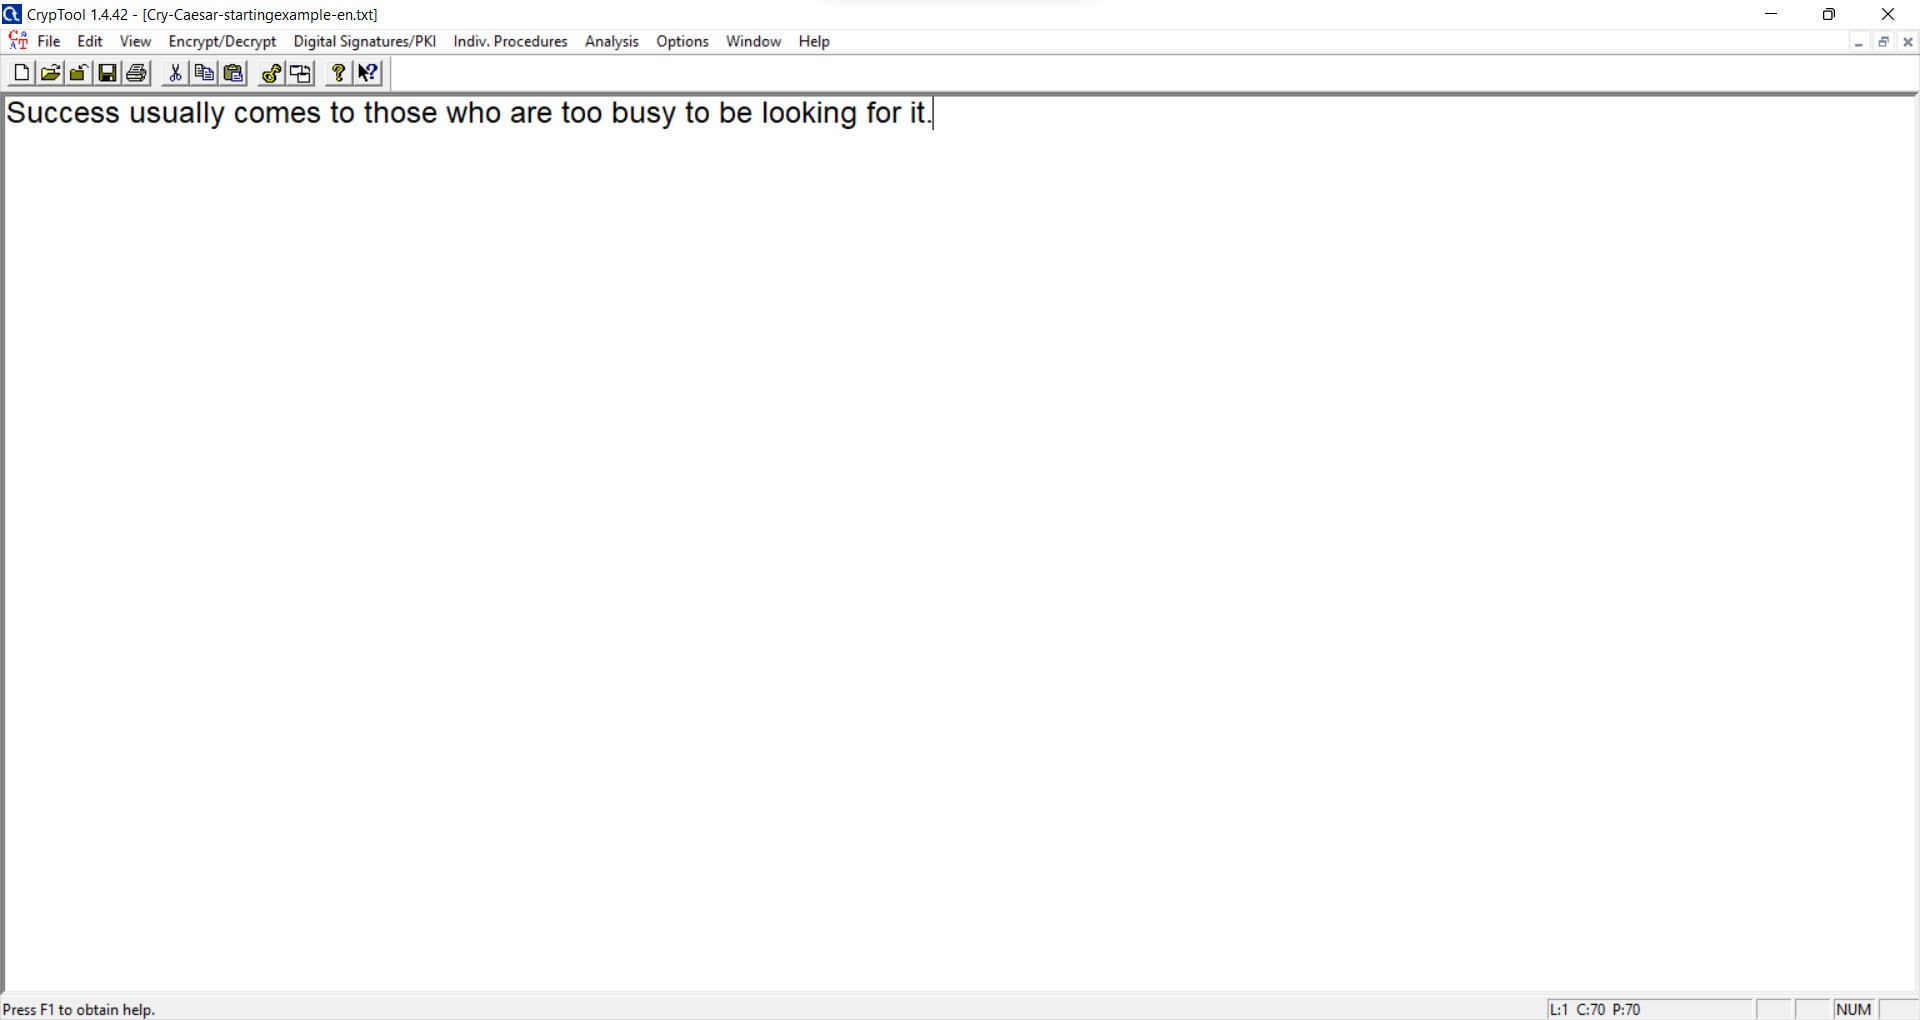
\includegraphics[width=0.75\textwidth]{figures/3aa.jpg}
    \caption
	{}
    \label{fig:fig1}
\end{figure}

\begin{figure}[H]
    \centering
    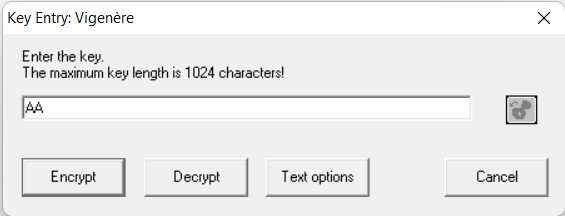
\includegraphics[width=0.75\textwidth]{figures/3ab.jpg}
    \caption
	{}
    \label{fig:fig1}
\end{figure}

\begin{figure}[H]
    \centering
    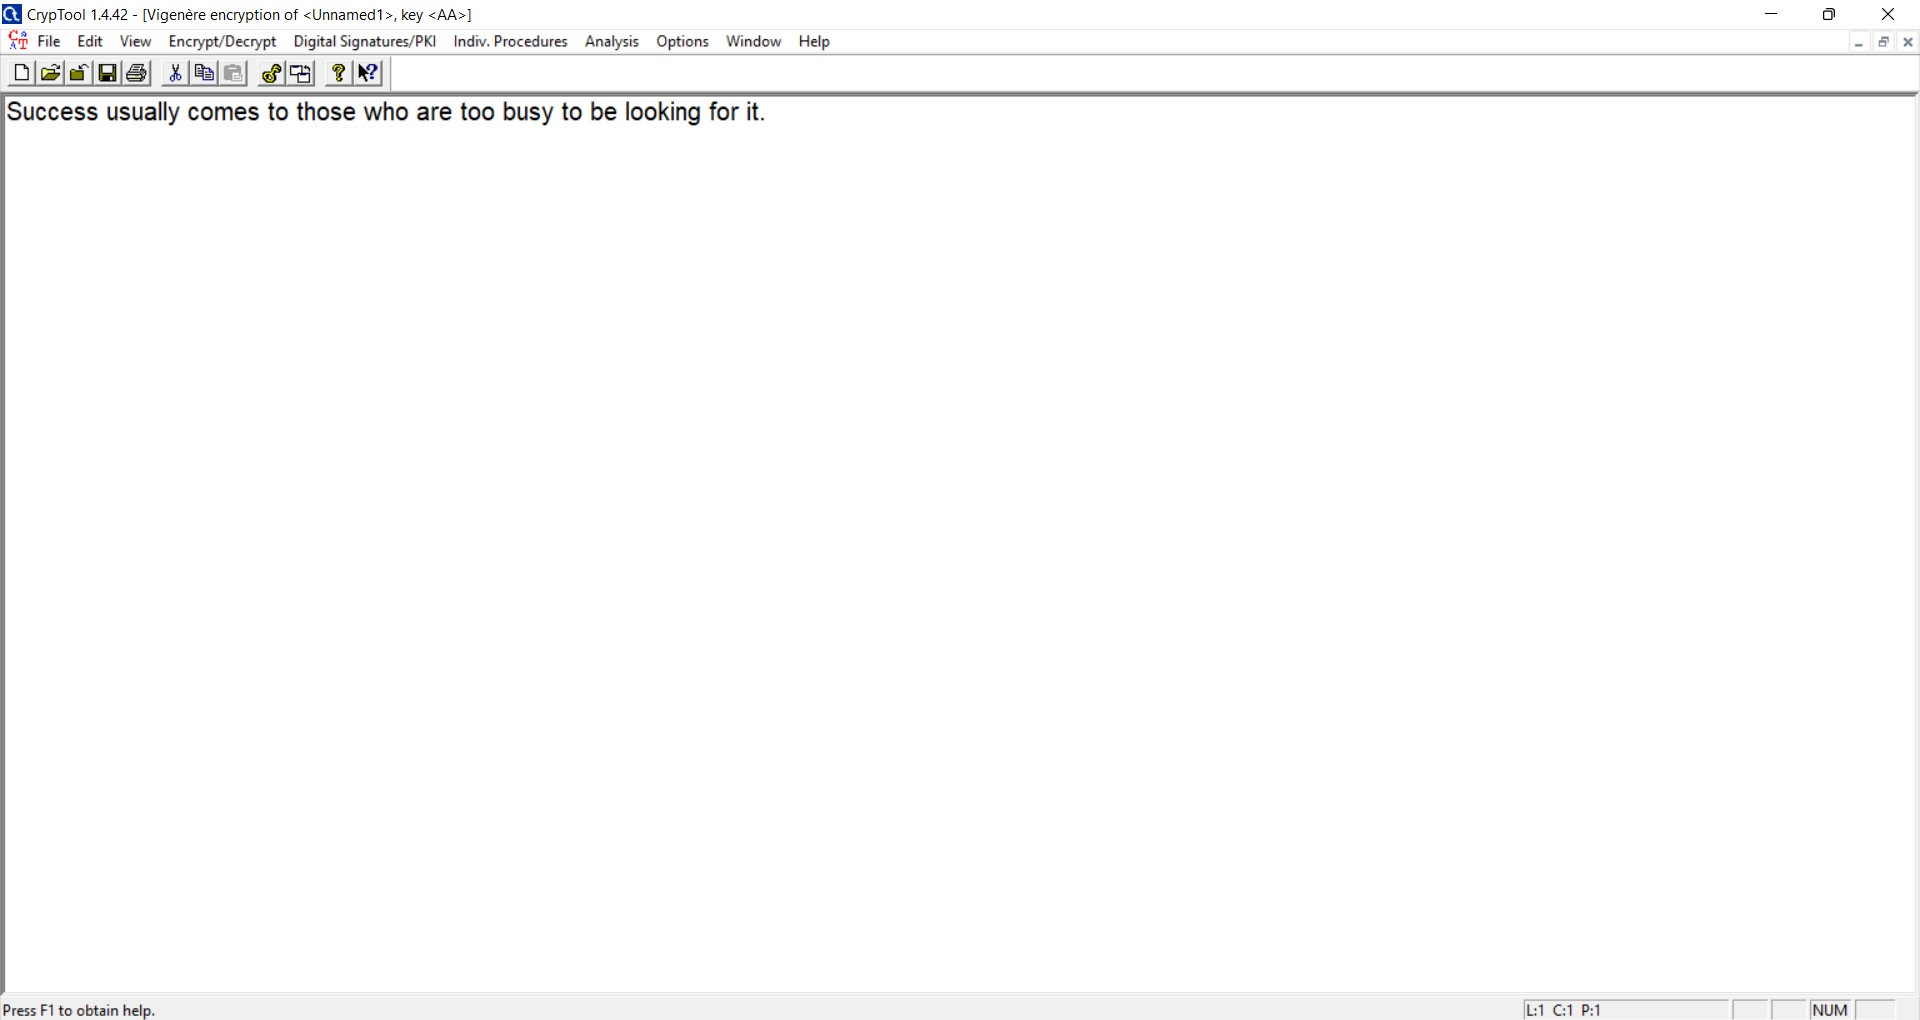
\includegraphics[width=0.75\textwidth]{figures/3ac.jpg}
    \caption
	{}
    \label{fig:fig1}
\end{figure}

\subsubsection{\lr{b}}
مشابه قسمت قبل (صرفا تغییر کلید) داریم:
\begin{latin}
$
ALIREZA\:\:ABREHFOROUSH \Rightarrow key = ALIREZAABREHFOROUSH
$
\end{latin}

\begin{latin}
% Please add the following required packages to your document preamble:
% \usepackage{graphicx}
\begin{table}[H]
\centering
\resizebox{\columnwidth}{!}{%
\begin{tabular}{|c|c|c|c|c|c|c|c|c|c|c|c|c|c|c|c|c|c|c|c|c|c|c|c|c|c|c|c|c|c|c|c|c|c|c|c|c|c|c|c|c|c|c|c|c|c|c|c|c|c|c|c|c|c|c|c|c|c|c|c|c|c|c|c|c|c|c|c|c|c|}
\hline
key    & A & l & i & r & e & z & a &  & a & b & r & e & h & f & o &  & r & o & u & s & h &  & a & l &  & i & r & e & z & a &  & a & b & r &  & e & h & f &  & o & r & o &  & u & s & h & a &  & l & i &  & r & e &  & z & a & a & b & r & e & h &  & f & o & r &  & o & u & . \\ \hline
x      & S & u & c & c & e & s & s &  & u & s & u & a & l & l & y &  & c & o & m & e & s &  & t & o &  & t & h & o & s & e &  & w & h & o &  & a & r & e &  & t & o & o &  & b & u & s & y &  & t & o &  & b & e &  & l & o & o & k & i & n & g &  & f & o & r &  & i & t & . \\ \hline
$E(x)$ & S & f & k & t & i & r & s &  & u & t & l & e & s & q & m &  & t & c & g & w & z &  & t & z &  & b & y & s & r & e &  & w & i & f &  & e & y & j &  & h & f & c &  & v & m & z & y &  & e & w &  & s & i &  & k & o & o & l & z & r & n &  & k & c & i &  & w & n & . \\ \hline
\end{tabular}%
}
\end{table}
\end{latin}
در نرم افزار \lr{CrypTool} به صورت زیر رمز می‌کنیم.
\begin{figure}[H]
    \centering
    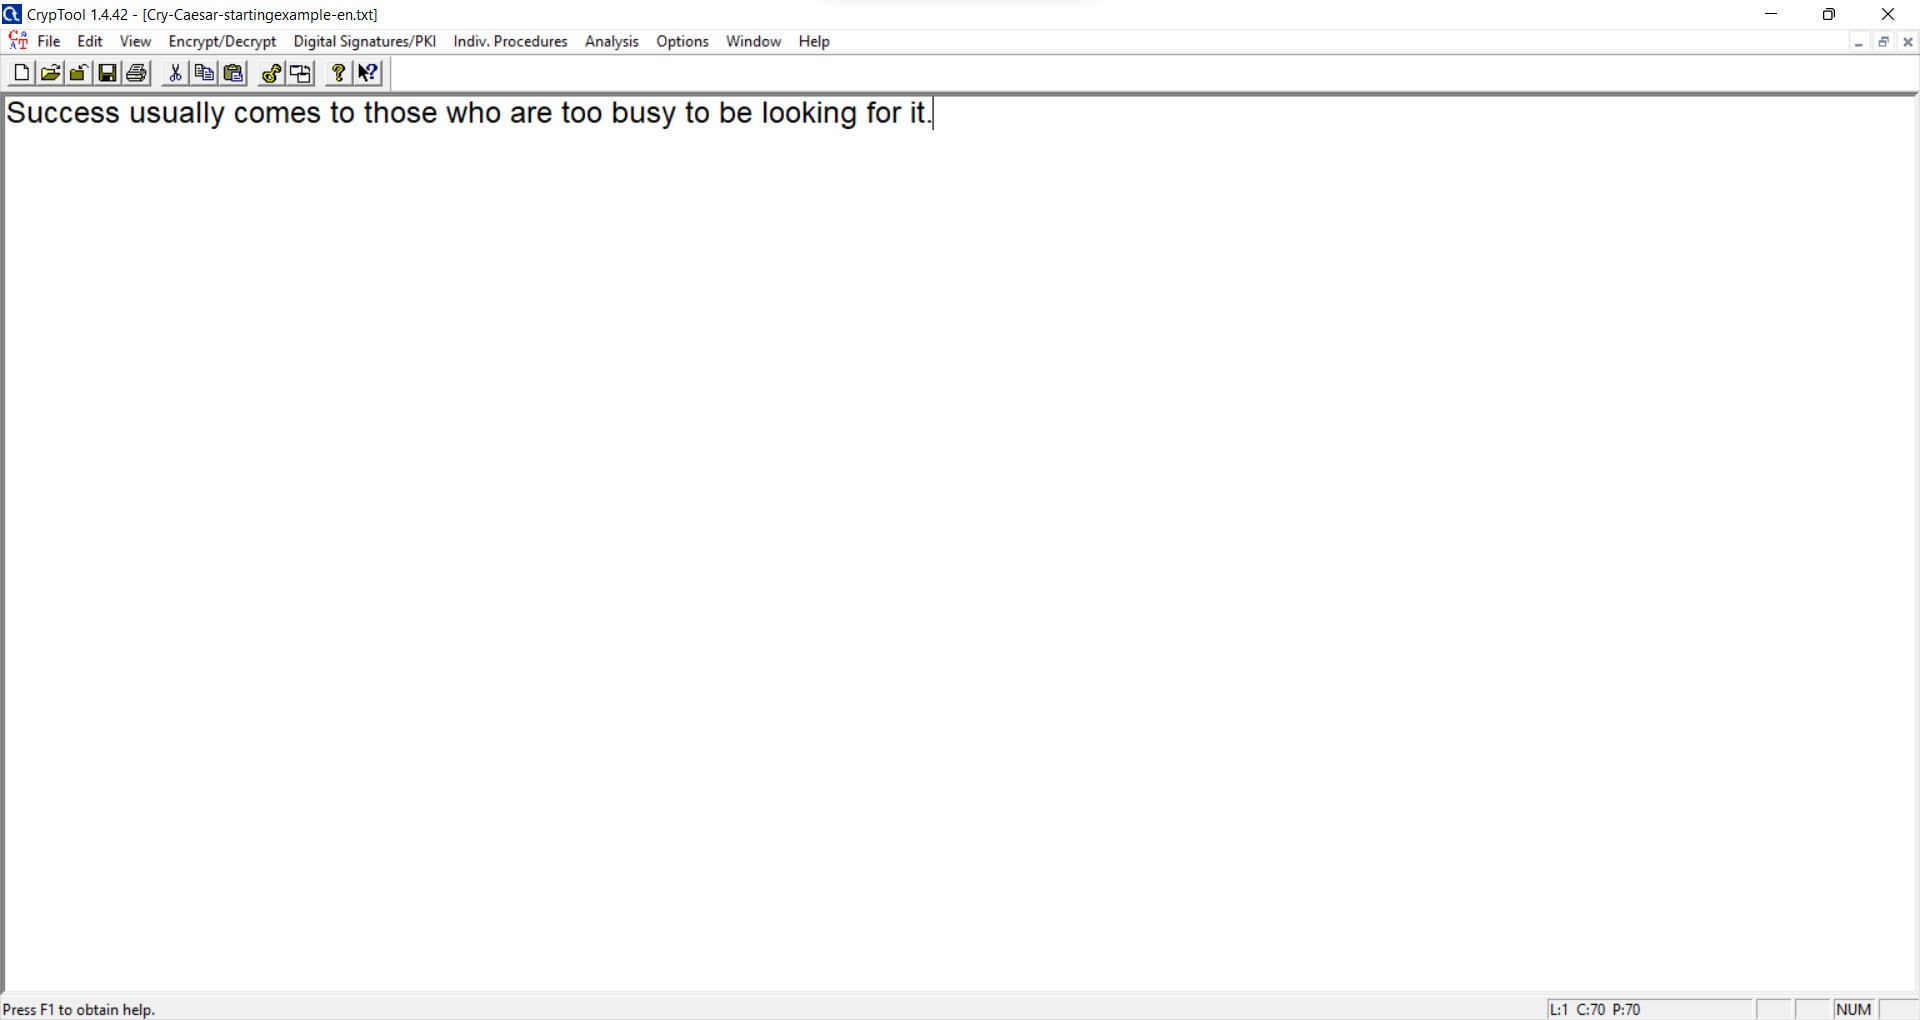
\includegraphics[width=0.75\textwidth]{figures/3ba.jpg}
    \caption
	{}
    \label{fig:fig1}
\end{figure}

\begin{figure}[H]
    \centering
    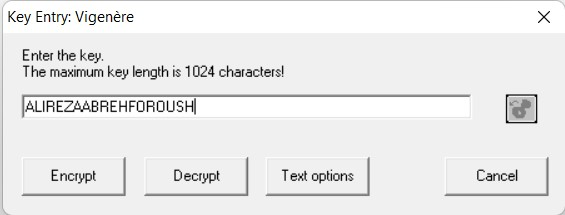
\includegraphics[width=0.75\textwidth]{figures/3bb.jpg}
    \caption
	{}
    \label{fig:fig1}
\end{figure}

\begin{figure}[H]
    \centering
    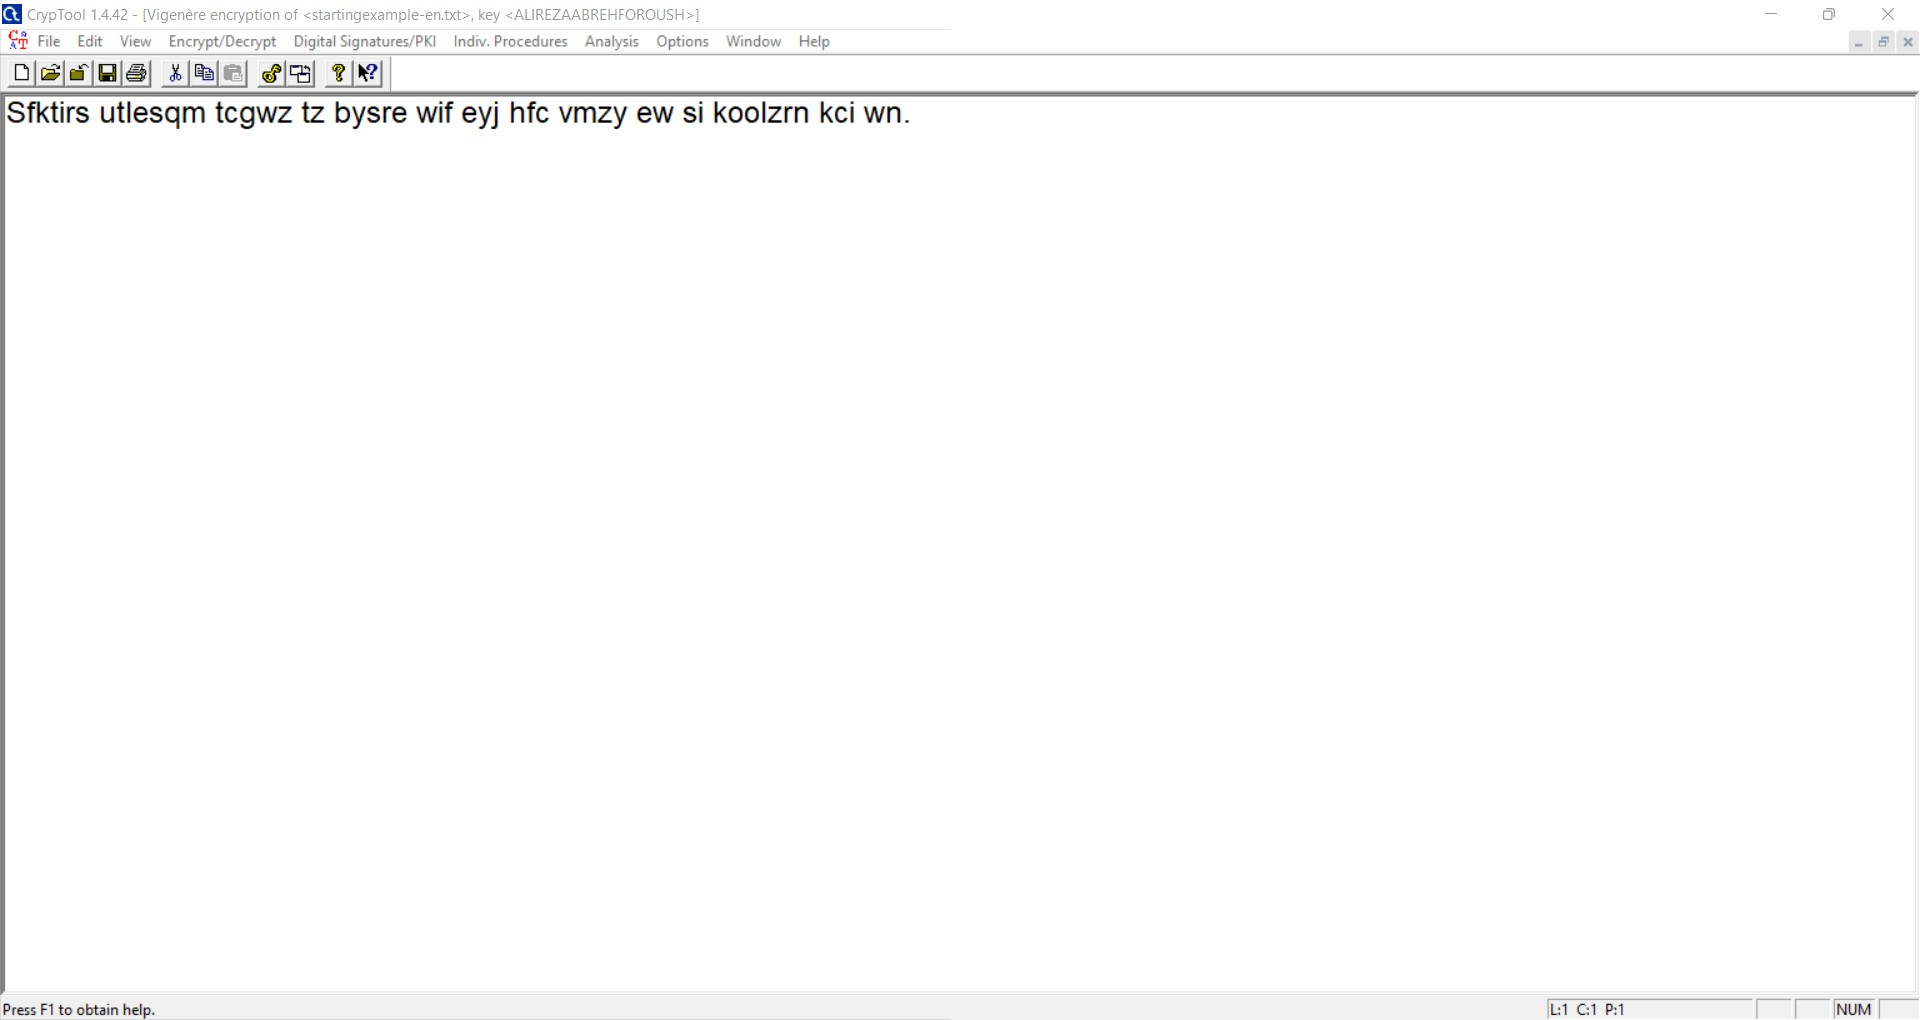
\includegraphics[width=0.75\textwidth]{figures/3bc.jpg}
    \caption
	{}
    \label{fig:fig1}
\end{figure}

\subsubsection{\lr{c}}
\begin{figure}[H]
    \centering
    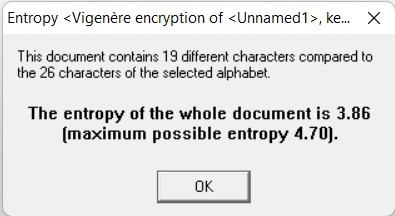
\includegraphics[width=0.75\textwidth]{figures/3ca.jpg}
    \caption
	{}
    \label{fig:fig1}
\end{figure}
\begin{figure}[H]
    \centering
    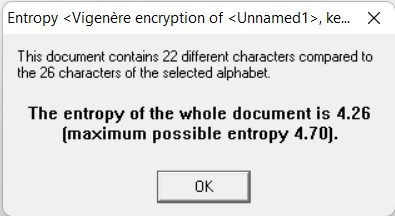
\includegraphics[width=0.75\textwidth]{figures/3cb.jpg}
    \caption
	{}
    \label{fig:fig1}
\end{figure}
آنتروپی در حالت اول و دوم به ترتیب برابر 3.86 و 4.26 است.
\begin{latin}
Entropy, in the context of cryptography, is related to random number generation, and more precisely, it refers to the “amount of unpredictable randomness” in a physical system. We call an entropy source the physical system that produces random signals.
\end{latin}
از آنجایی که در حالت دوم که طول کلید بیشتر است (کارکترهای متفاوت‌تری دارد) بی‌نظمی (\lr{randomness}) بیشتری وجود دارد، رمز امن‌تر است. در حالی که در حالت اول چون دو کاراکتر یکسان بودند صرفا از یک سطر (سطر اول که بدیهی هم هست) استفاده شده است و عبارت عملا رمز نشده است.




\subsection{}%4
در نرم افزار \lr{CrypTool} به صورت زیر رمزگشایی می‌کنیم. طول کلید (به طور پیشفرض) 5 است و کلید در \lr{Vigenère cipher} برابر \lr{SMILE} به دست می‌آید.
\begin{figure}[H]
    \centering
    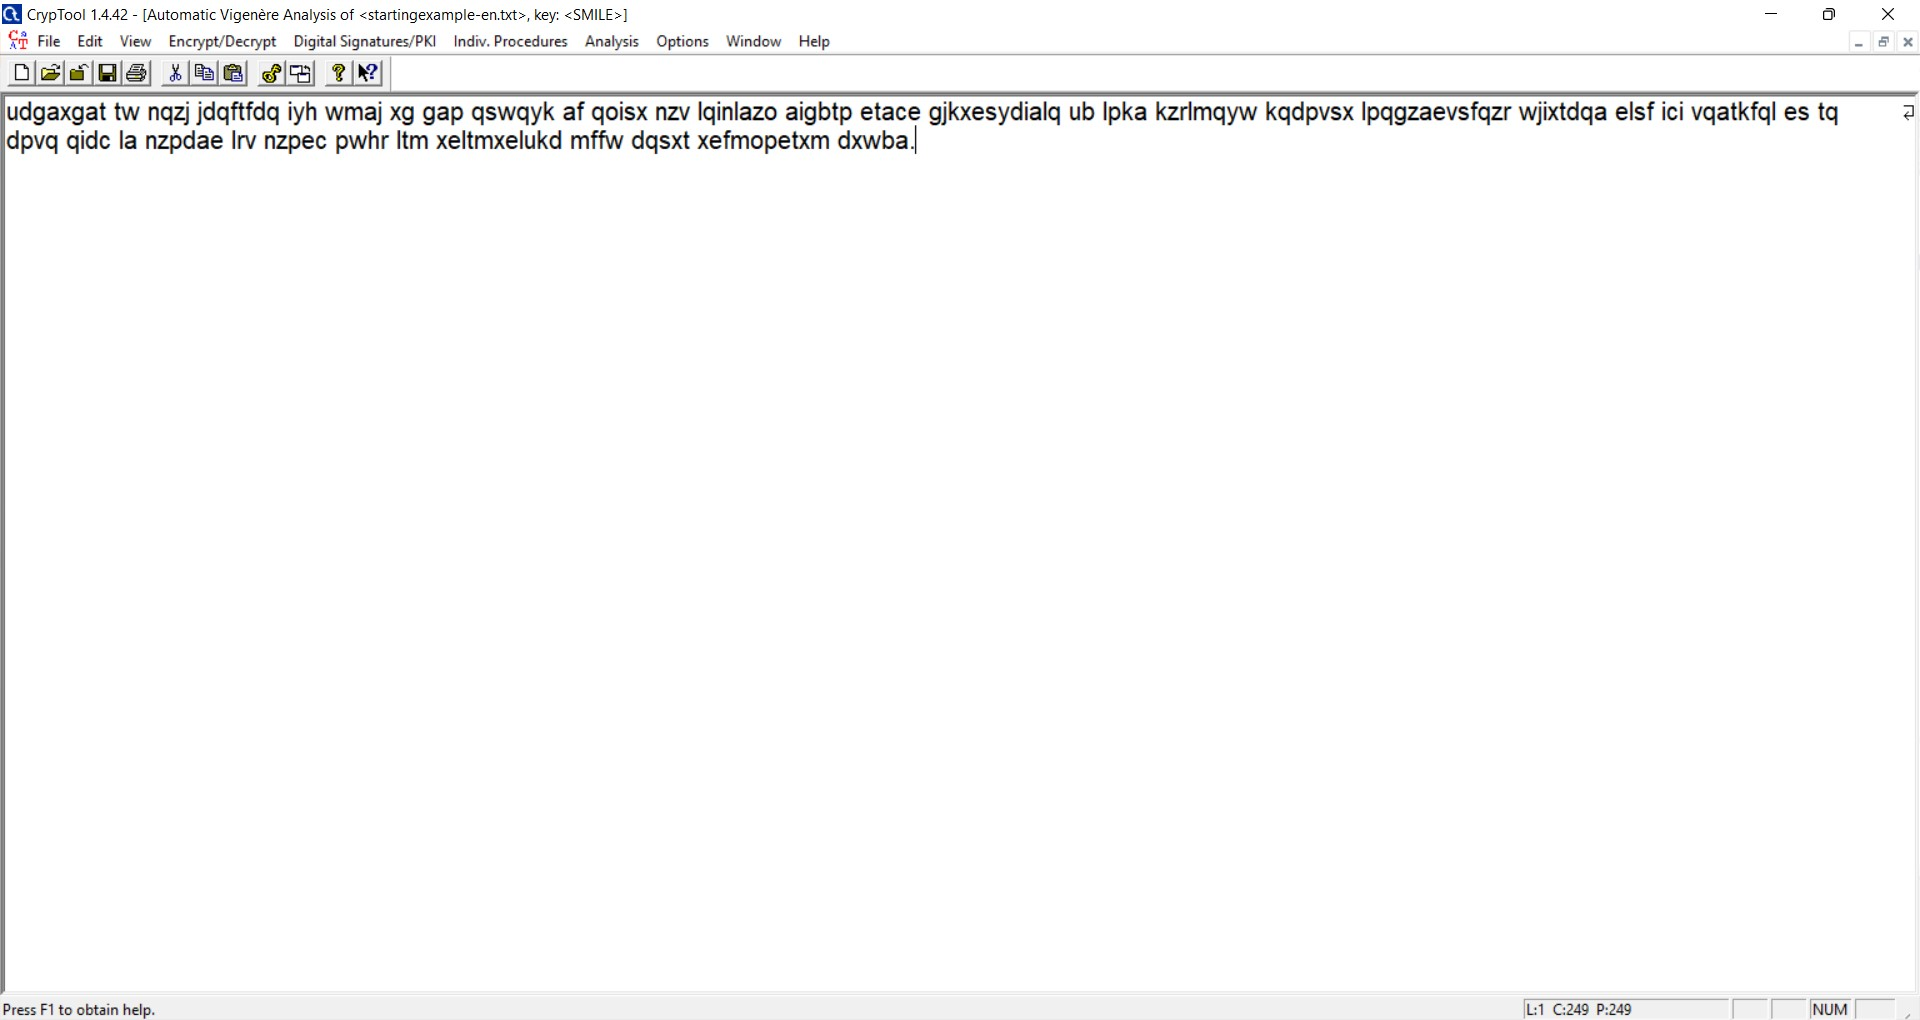
\includegraphics[width=0.75\textwidth]{figures/4a.jpg}
    \caption
	{}
    \label{fig:fig1}
\end{figure}

\begin{figure}[H]
    \centering
    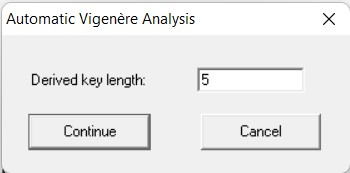
\includegraphics[width=0.75\textwidth]{figures/4b.jpg}
    \caption
	{}
    \label{fig:fig1}
\end{figure}

\begin{figure}[H]
    \centering
    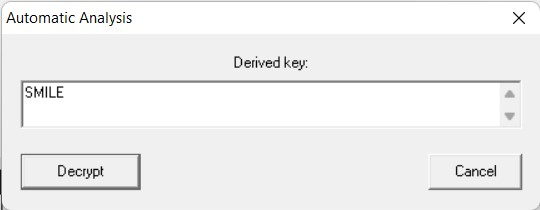
\includegraphics[width=0.75\textwidth]{figures/4c.jpg}
    \caption
	{}
    \label{fig:fig1}
\end{figure}

\begin{figure}[H]
    \centering
    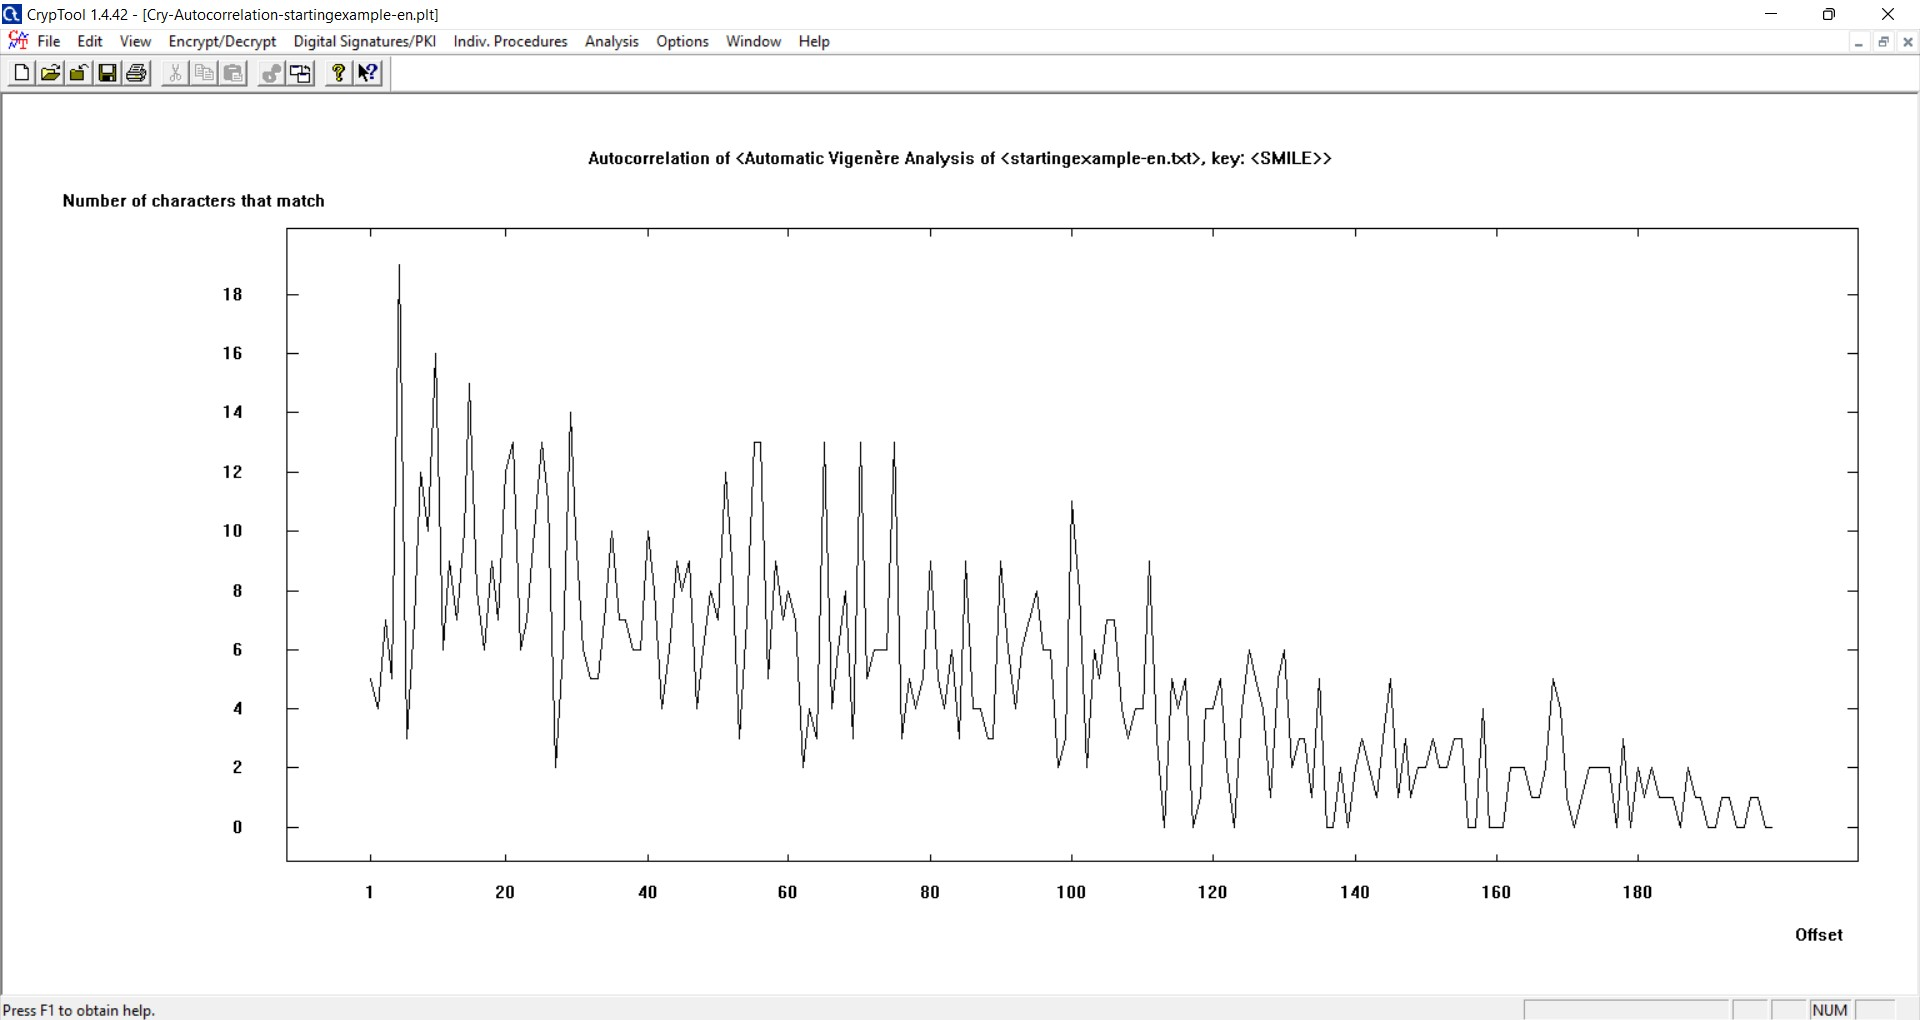
\includegraphics[width=0.75\textwidth]{figures/4d.jpg}
    \caption
	{}
    \label{fig:fig1}
\end{figure}

\begin{figure}[H]
    \centering
    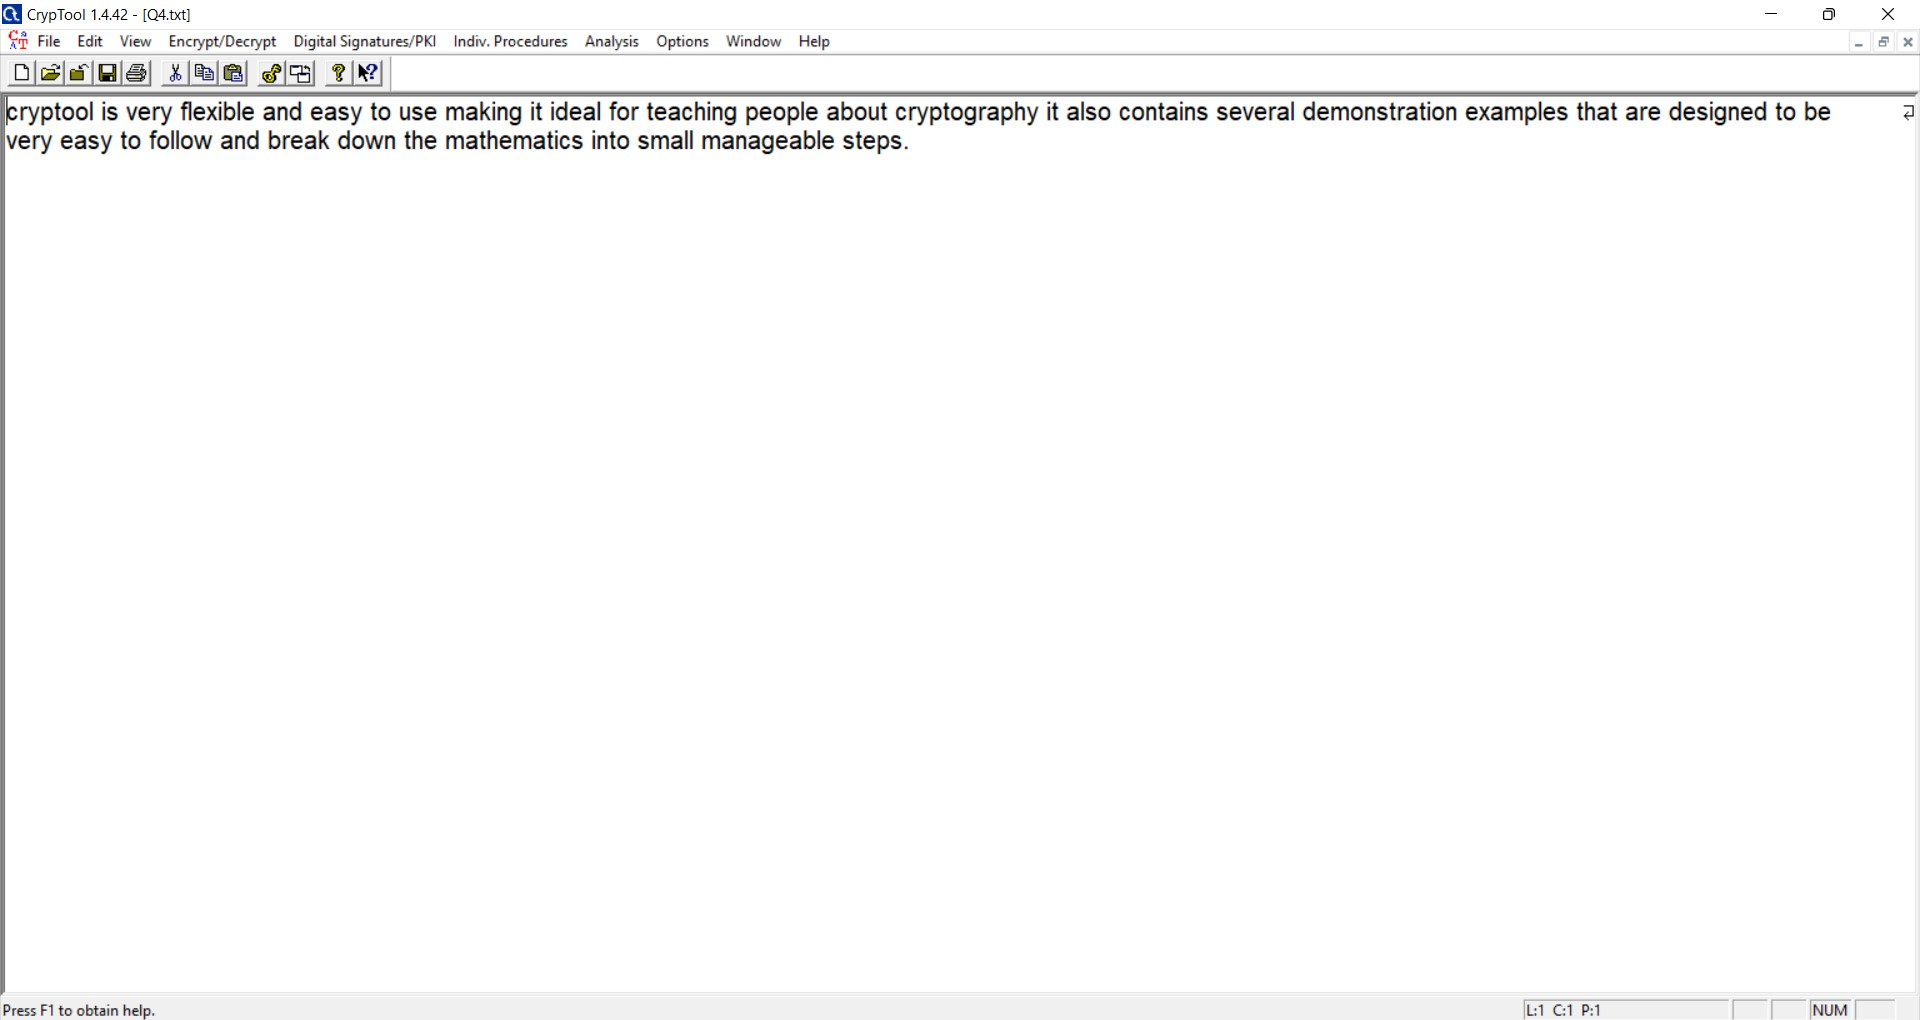
\includegraphics[width=0.75\textwidth]{figures/4e.jpg}
    \caption
	{}
    \label{fig:fig1}
\end{figure}
نمودار رسم شده \lr{autocorrelation} را نشان می‌دهد.  \lr{autocorrelation} یک متن را با نسخه‌های مختلف شیفت یافته‌ی آن (به طول یکسان) مقایسه می‌کند. در هر حالت کاراکترهایی که باهم \lr{match} می‌شوند (یکسان‌اند) را تعیین می‌کنیم. در نمودار رسم شده، تعداد کاراکترهای \lr{match}شده بر اساس تعداد واحد شیفت داده شده نمایش داده شده است. توجه شود که فقط حروف الفبای انتخاب شده (انگلیسی یا آلمانی برای مثال) تجزیه و تحلیل می‌شوند. همچنین تعداد جابه‌جایی‌ها به طول متن بستگی دارد (شما می‌توانید متنی متشکل از $n$ کاراکتر را حداکثر $n$ واحد جابجا کنید، سپس آن‌ها به نوعی زیر یکدیگر قرار می‌گیرند). به مثال زیر توجه کنید.
\begin{latin}
% Please add the following required packages to your document preamble:
% \usepackage{graphicx}
% \usepackage[table,xcdraw]{xcolor}
% If you use beamer only pass "xcolor=table" option, i.e. \documentclass[xcolor=table]{beamer}
\begin{table}[H]
\centering
\resizebox{\columnwidth}{!}{%
\begin{tabular}{|c|c|c|c|c|c|c|c|c|c|c|c|c|c|c|c|c|c|c|c|c|c|c|c|c|c|c|c|c|c|c|c|c|c|c|c|c|c|c|c|c|c|c|c|c|c|c|c|c|c|c|c|c|c|c|c|c|c|c|c|c|c|c|c|c|c|c|c|c|c|llllll}
\cline{1-70}
Orginal text & S & u & c & c & e & s & s                                  &                                    & u          & s & u & a & l & l & y &   & c & o & m & e & s &   & t & o &                                    & t & h & o & s & e &   & w                                  & h & o &                                    & a & r & e &   & t & o                                  & o                                  &   & b & u & s & y &   & t & o &   & b                                  & e &            & l & o & o & k & i & n & g &   & f & o & r &  & i & t & . &                      &                      &                      &                      &                      &                      \\ \cline{1-70}
Modified     & S & u & c & c & e & s & \cellcolor[HTML]{FFCCC9}\textbf{s} & \cellcolor[HTML]{FFCCC9}\textbf{u} & \textbf{s} & u & a & l & l & y & c & o & m & e & s & t & o & t & h & o & \cellcolor[HTML]{FFCCC9}\textbf{s} & e & w & h & o & a & r & \cellcolor[HTML]{FFCCC9}\textbf{e} & t & o & \cellcolor[HTML]{FFCCC9}\textbf{o} & b & u & s & y & t & \cellcolor[HTML]{FFCCC9}\textbf{o} & \cellcolor[HTML]{FFCCC9}\textbf{b} & e & l & o & o & k & i & n & g & f & \cellcolor[HTML]{FFCCC9}\textbf{o} & r & \textbf{i} & t & . &   &   &   &   &   &   &   &   &   &  &   &   &   &                      &                      &                      &                      &                      &                      \\ \cline{1-70}
Shifted by 6 &   &   &   &   &   &   & \cellcolor[HTML]{FFCCC9}\textbf{S} & \cellcolor[HTML]{FFCCC9}\textbf{u} & c          & c & e & s & s & u & s & u & a & l & l & y & c & o & m & e & \cellcolor[HTML]{FFCCC9}\textbf{s} & t & o & t & h & o & s & \cellcolor[HTML]{FFCCC9}\textbf{e} & w & h & \cellcolor[HTML]{FFCCC9}\textbf{o} & a & r & e & t & o & \cellcolor[HTML]{FFCCC9}\textbf{o} & \cellcolor[HTML]{FFCCC9}\textbf{b} & u & s & y & t & o & b & e & l & o & \cellcolor[HTML]{FFCCC9}\textbf{o} & k & \textbf{i} & n & g & f & o & r & i & t & . &   &   &   &  &   &   &   & \multicolumn{1}{c}{} & \multicolumn{1}{c}{} & \multicolumn{1}{c}{} & \multicolumn{1}{c}{} & \multicolumn{1}{c}{} & \multicolumn{1}{c}{} \\ \cline{1-70}
\end{tabular}%
}
\end{table}
\end{latin}
در این مثال در شیفت 6 واحد، تعداد کاراکترهای \lr{match}شده برابر 8 است.

\subsection{}%5

\subsubsection{\lr{a}}
\lr{plaintext} مذکور را با \lr{OTP Key} مذکور به شکل زیر با تکنیک \lr{one-time pad} رمز می‌کنیم.
\begin{figure}[H]
    \centering
    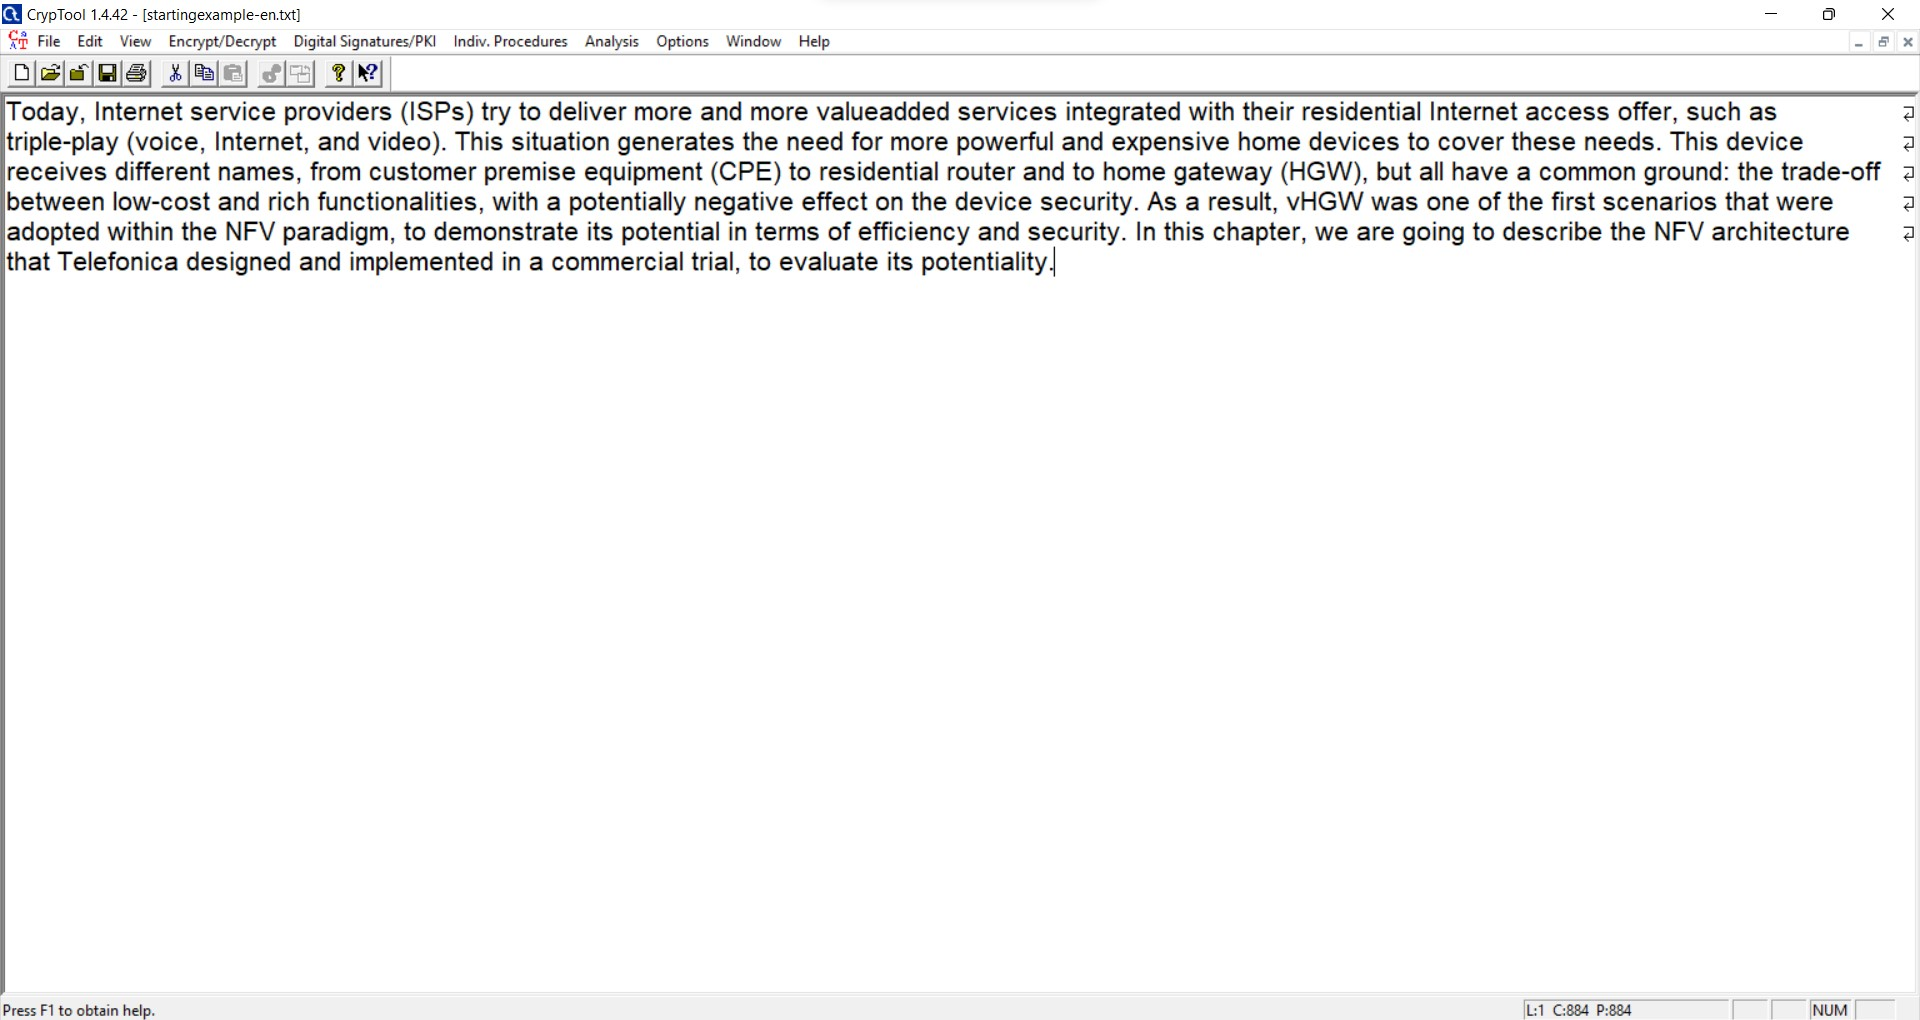
\includegraphics[width=0.75\textwidth]{figures/5a0.jpg}
    \caption
	{}
    \label{fig:fig1}
\end{figure}
\begin{figure}[H]
    \centering
    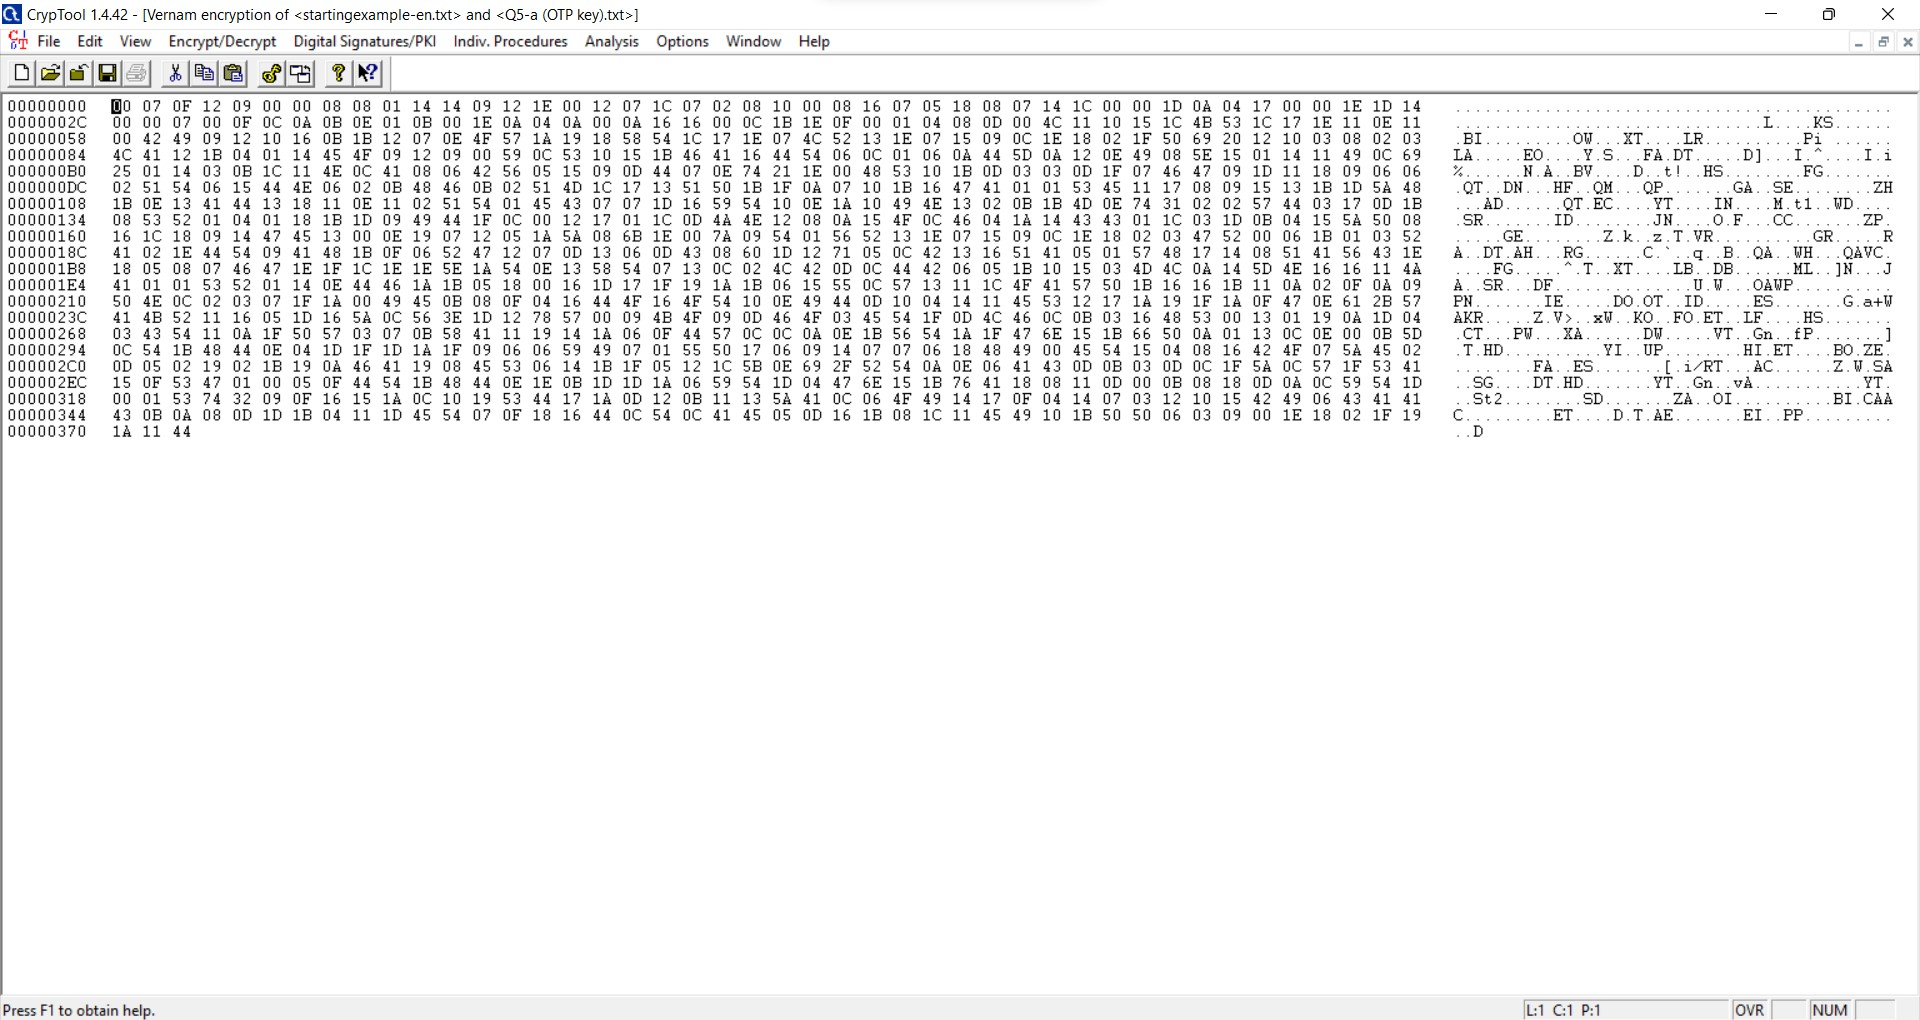
\includegraphics[width=0.75\textwidth]{figures/5a1.jpg}
    \caption
	{}
    \label{fig:fig1}
\end{figure}

\subsubsection{\lr{b}}
\lr{plaintext} مذکور را به شکل زیر با تکنیک \lr{one-time pad} رمز می‌کنیم. از آنجایی که طول کلید \lr{OTP} بایستی بزرگتر مساوی طول رشته‌ای که می‌خواهیم رمز کنیم باشد؛ به سه روش کلید \lr{OTP} را انتخاب می‌کنیم. یک بار کلید را برابر \lr{"alirezaabrehforoush"}، یک بار تکرار منظم حروف \lr{ALIREZAABREHFOROUSH} (یعنی با حفظ ترتیب کاراکترها را مطابق با بزرگ یا کوچک بودن یا کاراکتر نمادی بودنِ \lr{plain text} انتخاب می‌کنیم) و بار دیگر صرفا تکرار مکرر \lr{"Alireza Abrehforoush"}. هر سه حالت کلیدهای مذکور به پاسخ تکلیف پیوست شده است. (در اینجا فقط حالت اول آورده شده است)


\begin{figure}[H]
    \centering
    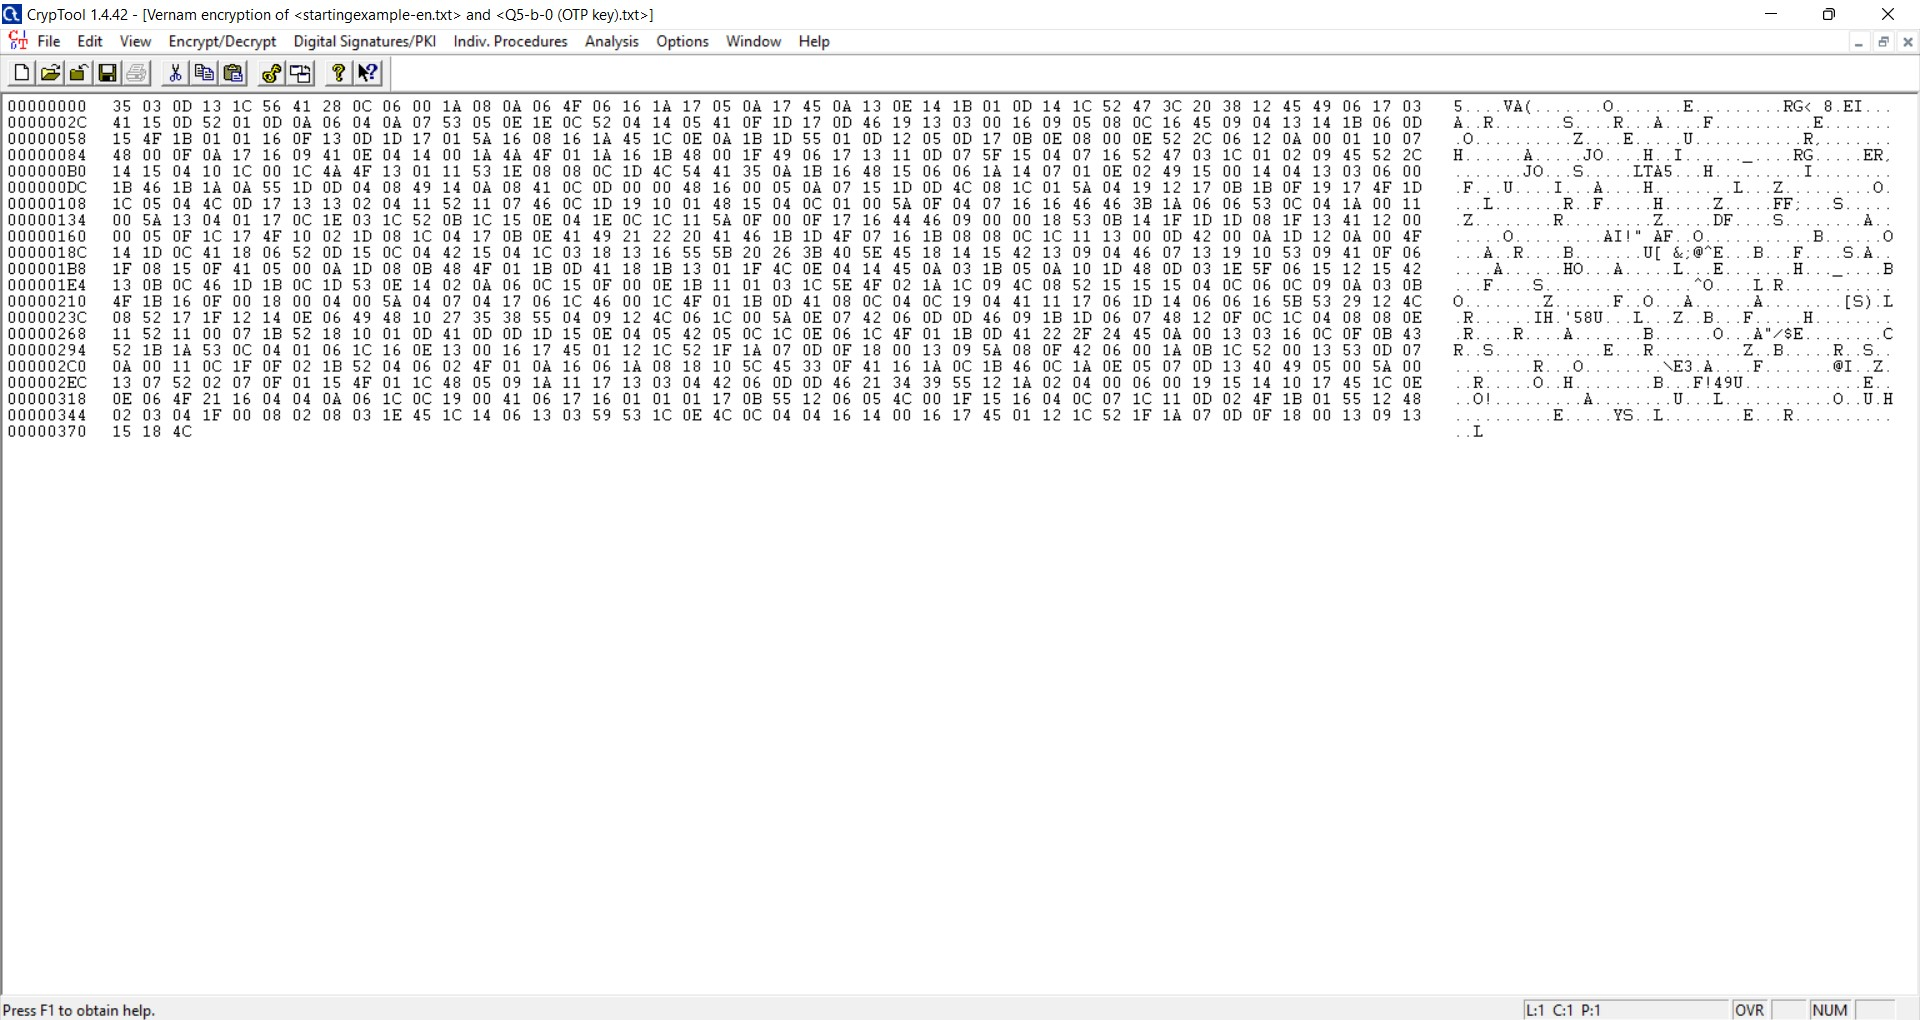
\includegraphics[width=0.75\textwidth]{figures/5b1.jpg}
    \caption
	{}
    \label{fig:fig1}
\end{figure}

\subsubsection{\lr{c}}
به شکل زیر تحلیل برای کشف کلید \lr{OTP} به ترتیب برای قسمت \lr{a} و \lr{b} انجام می‌شود.
\begin{figure}[H]
    \centering
    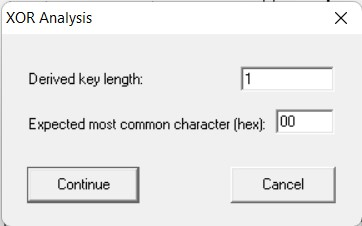
\includegraphics[width=0.75\textwidth]{figures/5c1.jpg}
    \caption
	{}
    \label{fig:fig1}
\end{figure}
\begin{figure}[H]
    \centering
    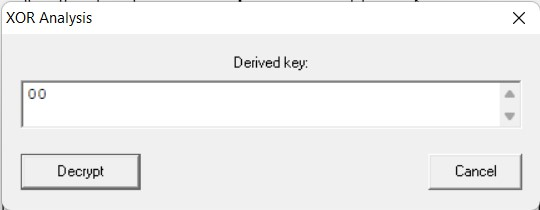
\includegraphics[width=0.75\textwidth]{figures/5c2.jpg}
    \caption
	{}
    \label{fig:fig1}
\end{figure}
\begin{figure}[H]
    \centering
    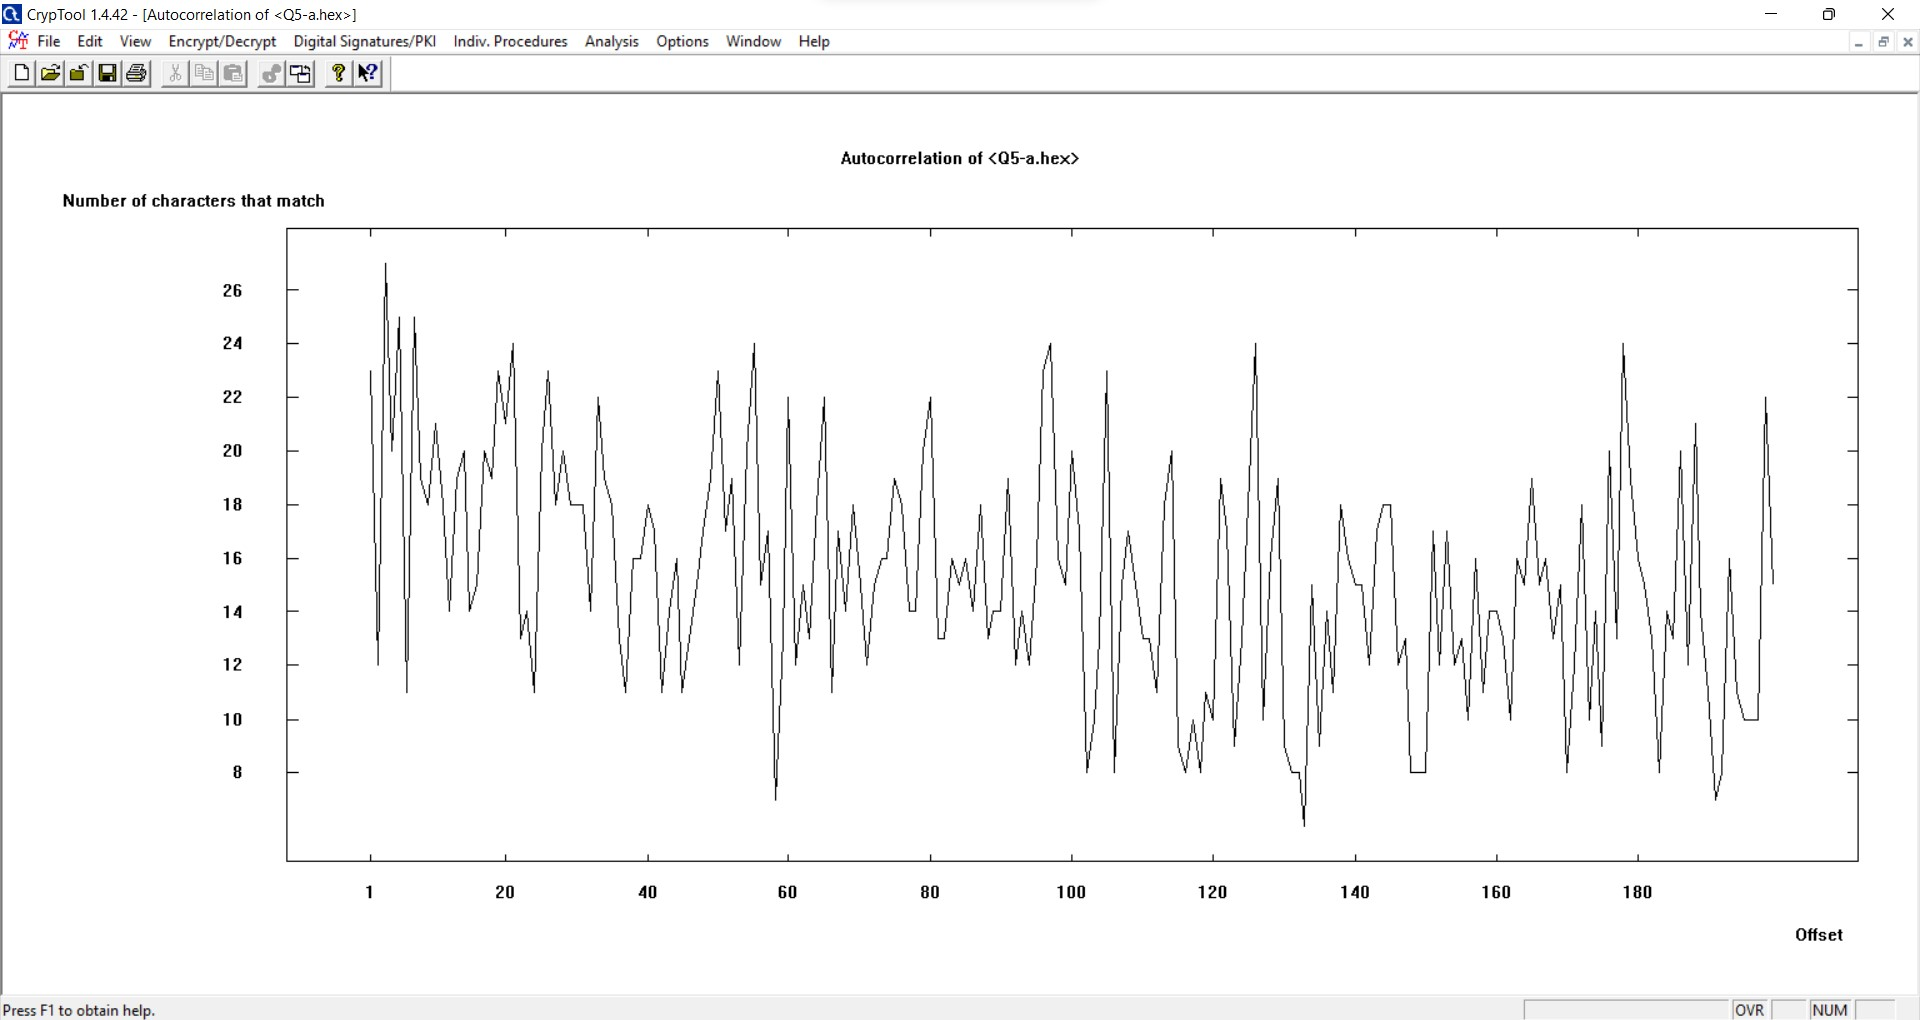
\includegraphics[width=0.75\textwidth]{figures/5c3.jpg}
    \caption
	{}
    \label{fig:fig1}
\end{figure}



\begin{figure}[H]
    \centering
    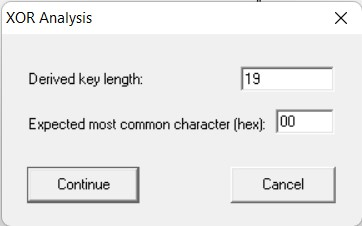
\includegraphics[width=0.75\textwidth]{figures/5c4.jpg}
    \caption
	{}
    \label{fig:fig1}
\end{figure}
\begin{figure}[H]
    \centering
    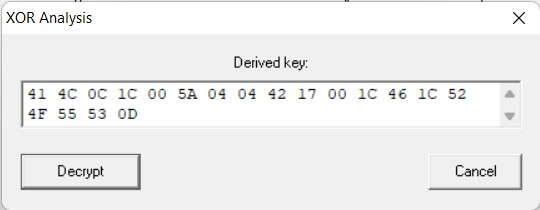
\includegraphics[width=0.75\textwidth]{figures/5c5.jpg}
    \caption
	{}
    \label{fig:fig1}
\end{figure}
\begin{figure}[H]
    \centering
    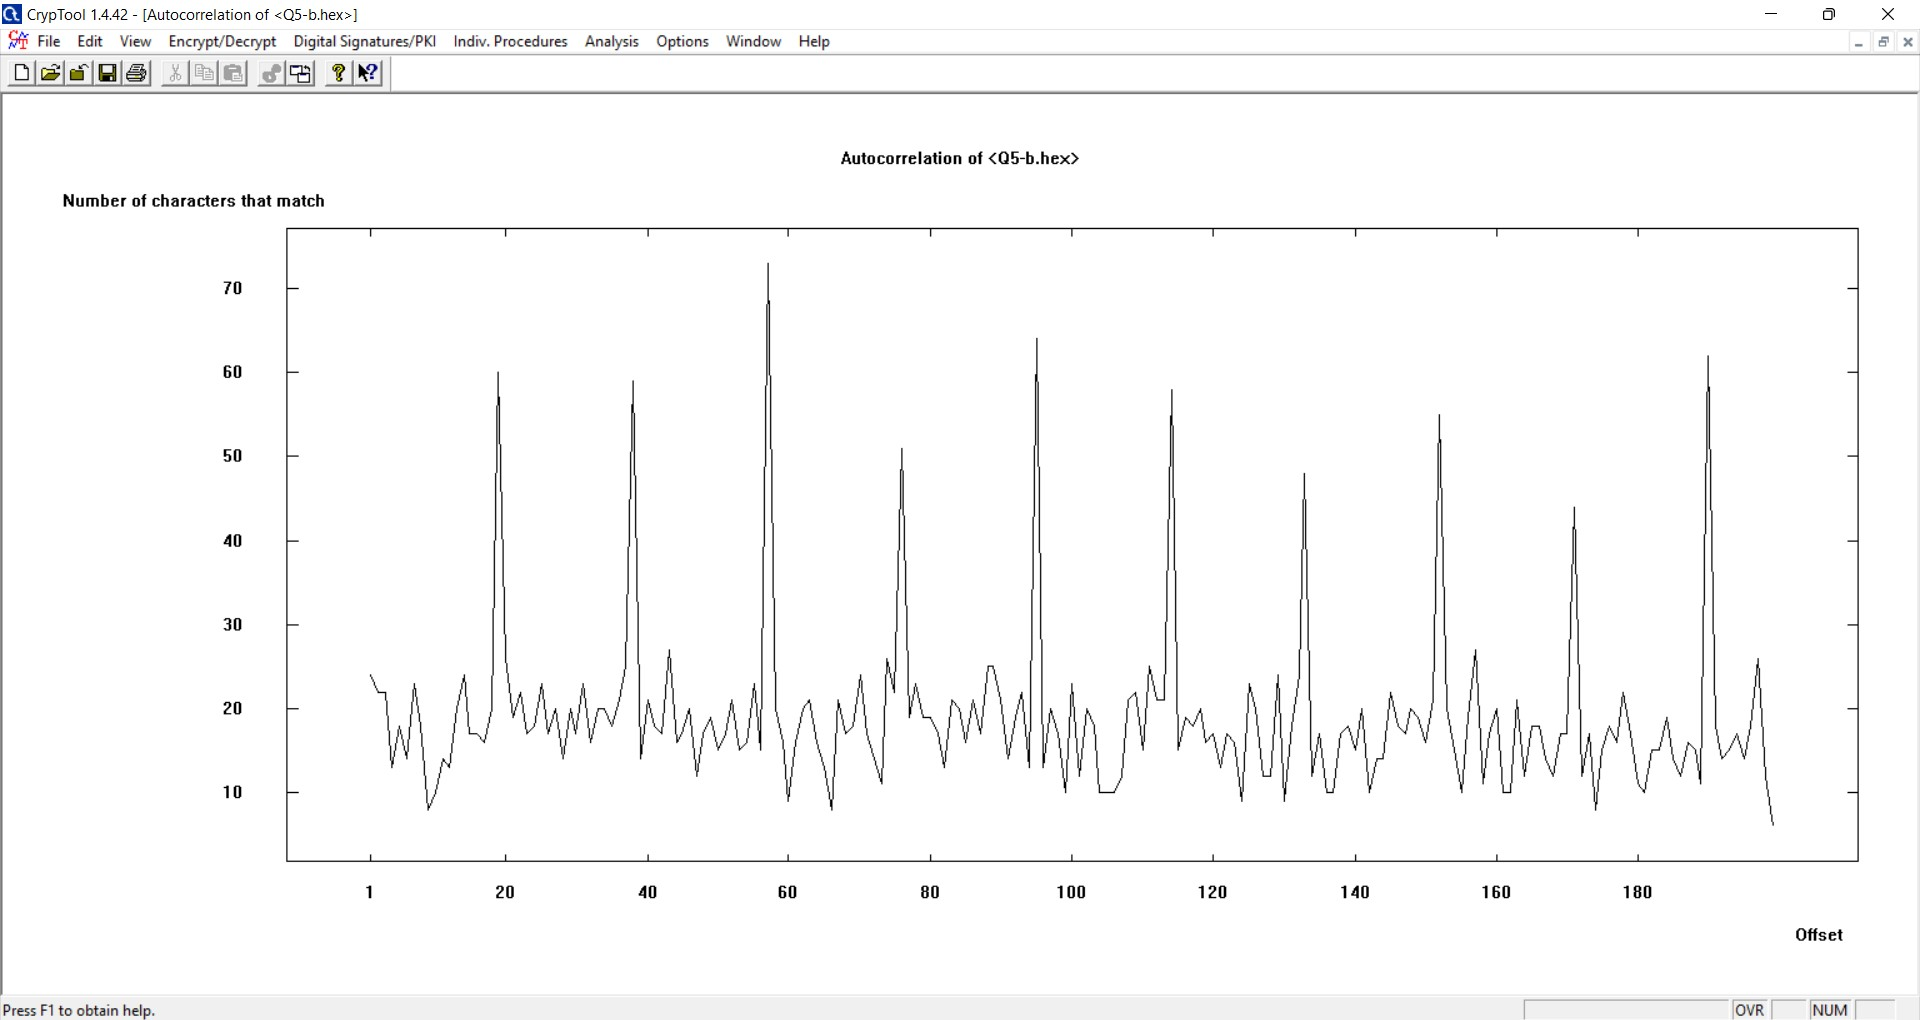
\includegraphics[width=0.75\textwidth]{figures/5c6.jpg}
    \caption
	{}
    \label{fig:fig1}
\end{figure}



همانطور که مشاهده می‌کنیم در حالت دوم که کلید دارای عبارات و کاراکترهای تکراری است طول کلید به درستی حدس زده شده است و همجنین قسمت‌هایی از کلید به درستی تشخیص داده شده است. پس امنیت پایین‌تری دارد.


\subsection{}
در نرم افزار \lr{CrypTool} به صورت زیر رمزگشایی می‌کنیم.
\begin{figure}[H]
    \centering
    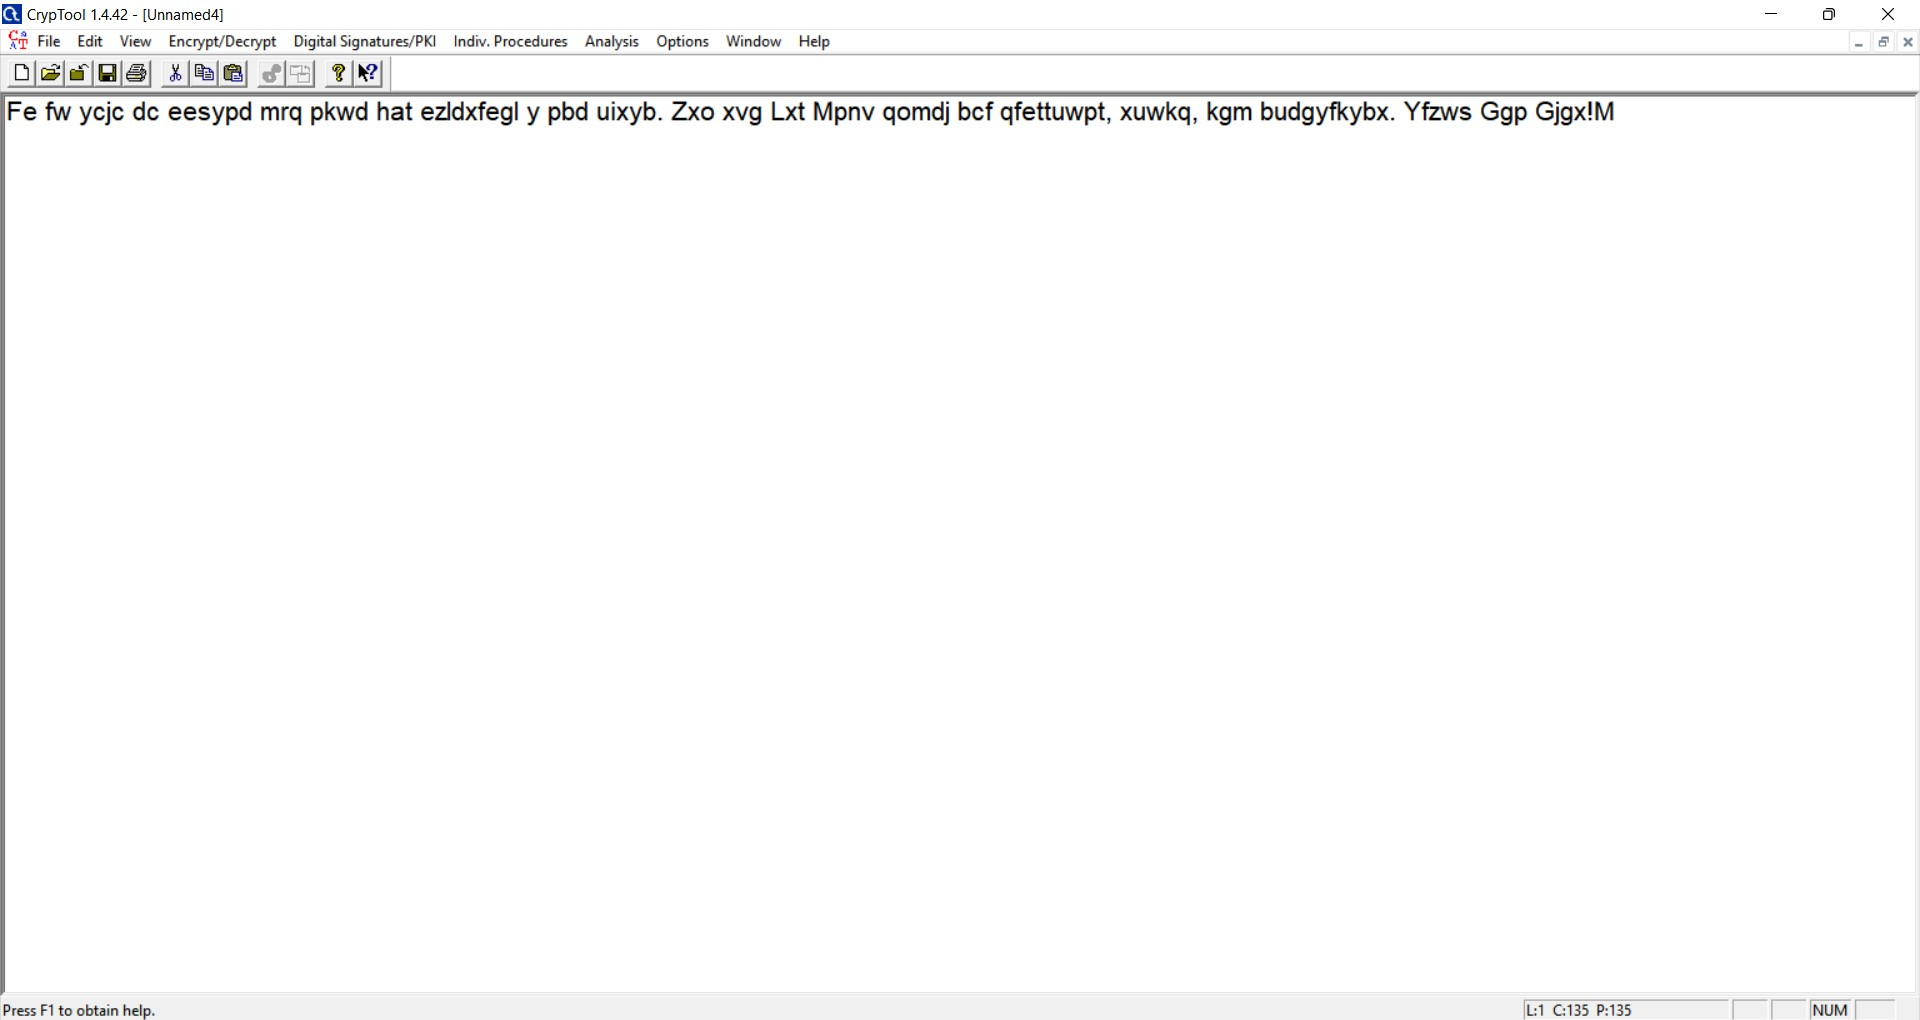
\includegraphics[width=0.75\textwidth]{figures/6a0.jpg}
    \caption
	{}
    \label{fig:fig1}
\end{figure}
\begin{figure}[H]
    \centering
    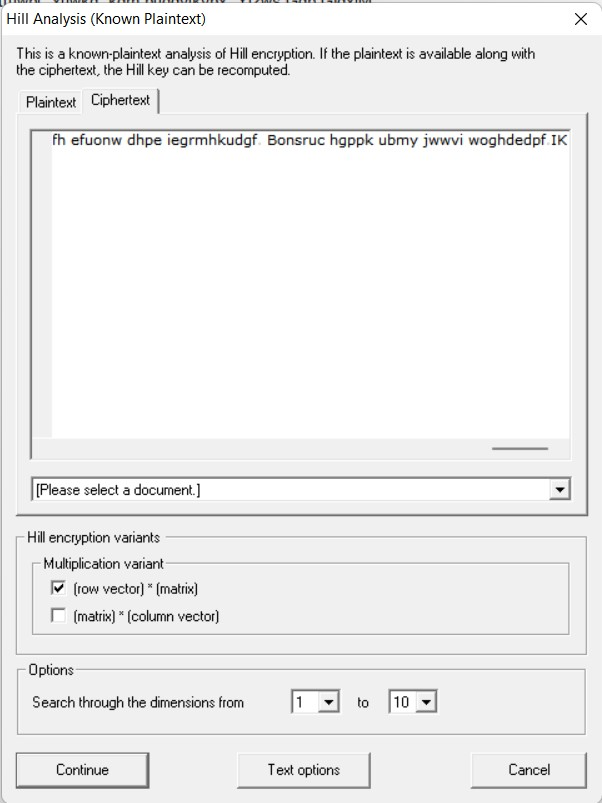
\includegraphics[width=0.75\textwidth]{figures/6a1.jpg}
    \caption
	{}
    \label{fig:fig1}
\end{figure}
\begin{figure}[H]
    \centering
    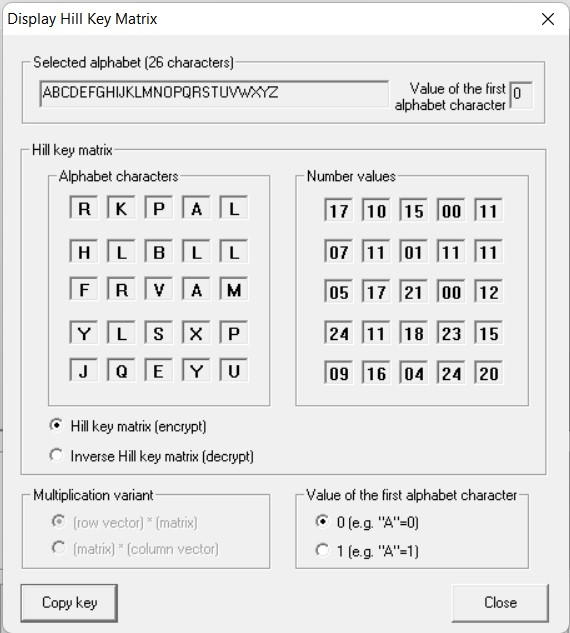
\includegraphics[width=0.75\textwidth]{figures/6a2.jpg}
    \caption
	{}
    \label{fig:fig1}
\end{figure}
\begin{figure}[H]
    \centering
    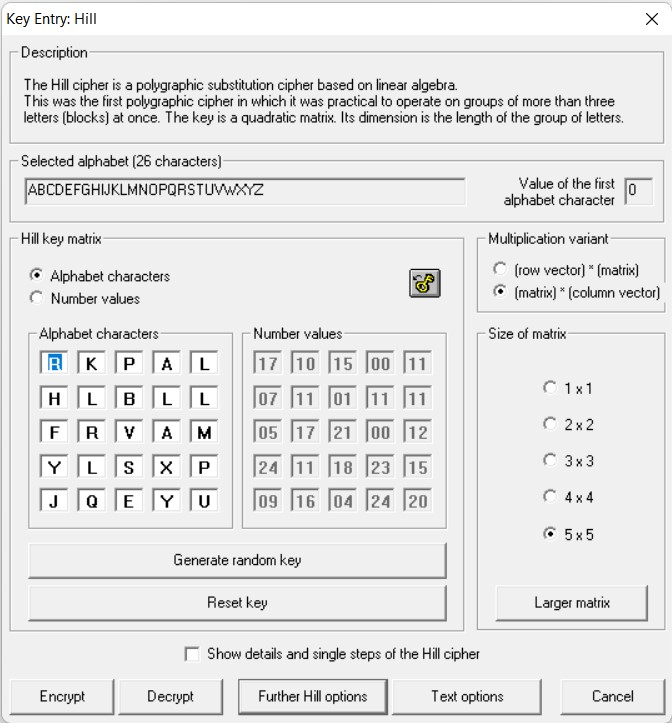
\includegraphics[width=0.75\textwidth]{figures/6a3.jpg}
    \caption
	{}
    \label{fig:fig1}
\end{figure}
\begin{figure}[H]
    \centering
    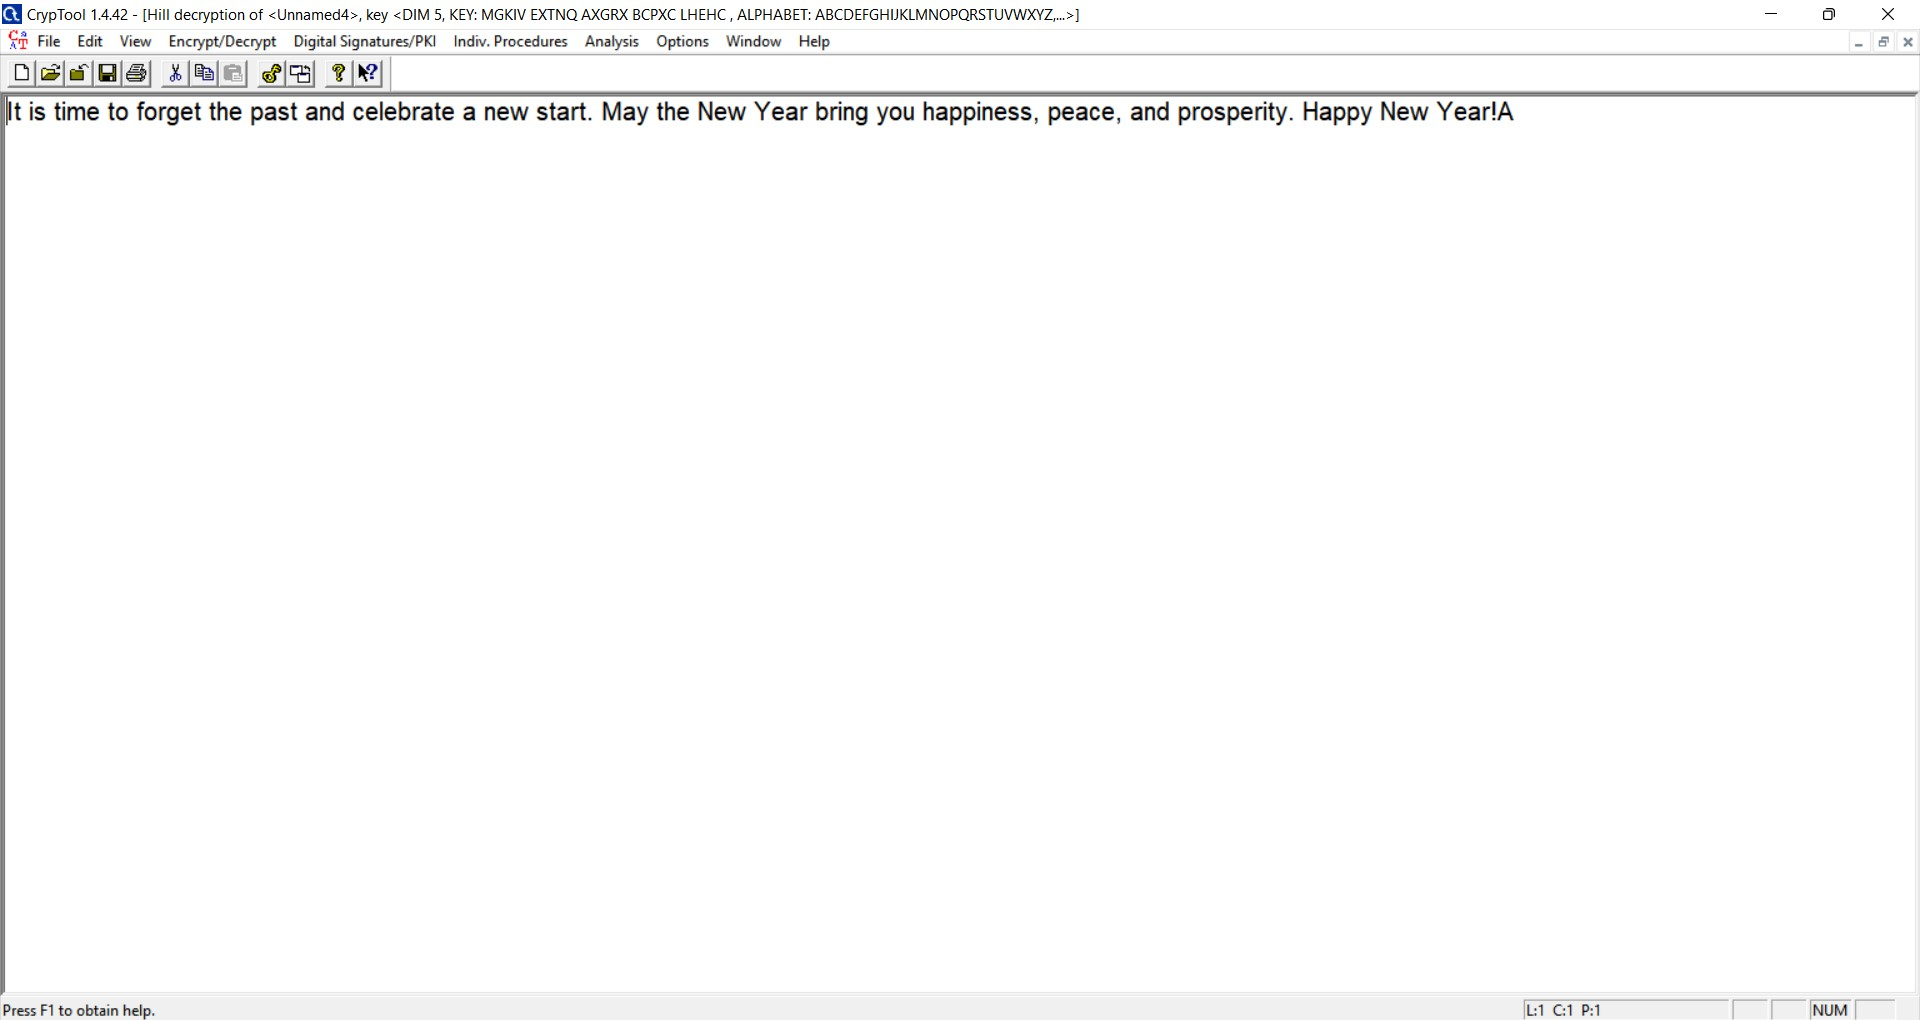
\includegraphics[width=0.75\textwidth]{figures/6a4.jpg}
    \caption
	{}
    \label{fig:fig1}
\end{figure}
پیام محرمانه \lr{"It is time to forget the past and celebrate a new start. May the New Year bring you happiness, peace, and prosperity. Happy New Year!A"} است.

%\begin{latin}
%\lstinputlisting{sources/p2.m}
%\end{latin}


%%%%%%%%%%%%%%%%%%%%%%%%%%%%%%%%%%%
%%%%%%%%%%%%%%%%%%%%%%%%%%%%%%%%%%%
%%%%%%%%%%%%%%%%%%%%%%%%%%%%%%%%%%%

%------------------------------------------------------------------------------------------


\subsection*{منابع}
\renewcommand{\subsection}[2]{}%
\begin{thebibliography}{99} % assumes less than 100 references
%چنانچه مرجع فارسی نیز داشته باشید باید دستور فوق را فعال کنید و مراجع فارسی خود را بعد از این دستور وارد کنید


\begin{LTRitems}

\resetlatinfont

\bibitem{b1}
\end{LTRitems}

\end{thebibliography}


\end{document}
